% IronBuddy 课程结项报告
% 编译：xelatex main.tex（两遍生成目录）
% 字体：ctex 默认（fandol 或系统 Noto CJK），不显式指定避免环境差异

\documentclass[UTF8,a4paper,12pt]{ctexart}

\usepackage[margin=2.5cm]{geometry}
\usepackage{graphicx}
\usepackage{amsmath,amssymb}
\usepackage{booktabs}
\usepackage{array}
\usepackage{caption}
\usepackage{subcaption}
\usepackage{xcolor}
\usepackage{listings}
\usepackage{tikz}
\usepackage{algorithm}
\usepackage{algpseudocode}
\usepackage{hyperref}
\usetikzlibrary{arrows.meta,positioning,shapes.geometric,fit,calc}

% 使用系统 Noto CJK，避免默认 Fandol 字体缺少姓名中的生僻字。
\setCJKmainfont{Noto Serif CJK SC}
\setCJKsansfont{Noto Sans CJK SC}
\setCJKmonofont{Noto Sans Mono CJK SC}
\hypersetup{
  colorlinks=true,
  linkcolor=black,
  urlcolor=blue!60!black,
  citecolor=blue!60!black,
  pdftitle={IronBuddy 智能健身教练系统课程结项报告},
  pdfauthor={李浩瑄}
}

% 代码块样式
\lstset{
  basicstyle=\ttfamily\small,
  breaklines=true,
  frame=single,
  rulecolor=\color{gray!50},
  numbers=left,
  numberstyle=\tiny\color{gray},
  keywordstyle=\color{blue!70!black},
  commentstyle=\color{green!50!black},
  stringstyle=\color{orange!70!black},
  showstringspaces=false
}

% 章节间距收紧
\linespread{1.25}
\setlength{\parskip}{0.4em}

% 自定义命令
\newcommand{\code}[1]{\nolinkurl{#1}}
\newcommand{\term}[1]{\textbf{#1}}

\begin{document}

\pagenumbering{gobble}
\pagestyle{empty}

% ============================================================
% 浙江大学实验报告封面
% ============================================================
\begin{titlepage}
    \centering
    \vspace*{1.2cm}

    % 校徽
    
\includegraphics[width=3.4cm]{封面/logo.png}\\[0.6cm]

    % 毛笔体"浙江大学实验报告"标题图
    
\includegraphics[width=0.78\textwidth]{封面/head.jpg}\\[2.2cm]

    % 实验主题副标题
    {\Large\bfseries IronBuddy 智能健身教练系统}\\[0.4em]
    {\large 基于 RK3399ProX 的双模态交互系统的工程实现}\\[2.6cm]

    % 信息表
    {\Large
    \renewcommand{\arraystretch}{1.7}
    \begin{tabular}{rl}
        \textbf{课程名称：} & \underline{\makebox[260pt]{嵌入式系统课程设计}} \\
        \textbf{实验名称：} & \underline{\makebox[260pt]{IronBuddy 智能健身教练系统}} \\
        \textbf{姓\hspace{2em}名：} & \underline{\makebox[260pt]{李浩瑄}} \\
        \textbf{学\hspace{2em}号：} & \underline{\makebox[260pt]{3230105807}} \\
        \textbf{指导教师：} & \underline{\makebox[260pt]{杜歆}} \\
        \textbf{实验日期：} & \underline{\makebox[260pt]{\today}} \\
    \end{tabular}}

    \vfill
    {\small 项目仓库：\url{https://github.com/qqyyqq812/IronBuddy}}\\[0.4cm]
\end{titlepage}

\clearpage

\tableofcontents
\clearpage

\pagestyle{plain}
\pagenumbering{arabic}
\setcounter{page}{1}

\section*{摘要}
\addcontentsline{toc}{section}{摘要}

IronBuddy 是一个面向居家健身场景的嵌入式智能教练系统。项目关注的核心
问题是：摄像头能够看到动作姿态，却难以判断目标肌肉是否真正参与发力。
在深蹲、弯举这类训练中，两次动作的骨架轨迹可能接近，但目标肌激活、
代偿肌参与和训练刺激并不相同。系统因此把视觉姿态估计与表面肌电
（sEMG）放入同一条反馈链路，尝试同时判断动作形态、目标肌参与和代偿
趋势。

系统由 RK3399ProX 边缘计算节点、摄像头和麦克风等板端外设、ESP32 肌电
传输单元、贴片电极与穿戴固定结构、FSM/GRU 动作评估模块、语音交互、
Web 前端和后台记录接口组成。视觉侧提供关节角度、角速度和动作相位，
肌电侧通过 RMS 与 MVC 归一化描述目标肌和代偿肌的激活水平；两类信号
经过 Mid-Fusion 形成 7D 特征窗口，再由 CompensationGRU 给出标准、
代偿或不标准的动作质量判断。训练反馈不只统计完成次数，也围绕目标肌
激活、代偿情况和疲劳积分组织，更接近结果导向的训练记录方式。

在交互层面，系统通过语音唤醒、指令控制、DeepSeek 对话、训练总结和
本地数据库记录，减少运动过程中对触屏操作的依赖。长期记录、用户偏好
和周期性总结作为工程接口预留，属于后续扩展方向；真实 sEMG 连续输入、
语音现场稳定性与完整手测流程仍需继续复测。

\textbf{关键词}：嵌入式系统、边缘计算、表面肌电、人体姿态估计、多模态
融合、人机交互

\newpage

\clearpage
\section{研究背景与设计目标}

\subsection{从“看起来标准”到“真的练到了”}

居家健身系统近几年越来越常见，但大多数产品仍然把核心能力放在摄像头
姿态识别上。这个方向有其合理性：摄像头便宜、安装简单，人体骨架检测模型
也已经相对成熟。它能判断膝盖有没有内扣、手臂有没有抬到位、动作幅度
是否够大，因此适合承担第一层动作反馈。

问题在于，健身动作不只是一条外部轨迹。两个人做出几乎相同的深蹲姿态，
一个可能主要由股四头肌和臀肌发力，另一个可能更多依赖关节代偿和代偿肌
完成动作。
在摄像头眼里，这两种动作可能差别不大；但从训练效果和损伤风险看，它们
并不是同一类动作。也就是说，纯视觉系统能看到“形”，却看不到“力”。

\begin{figure}[htbp]
    \centering
    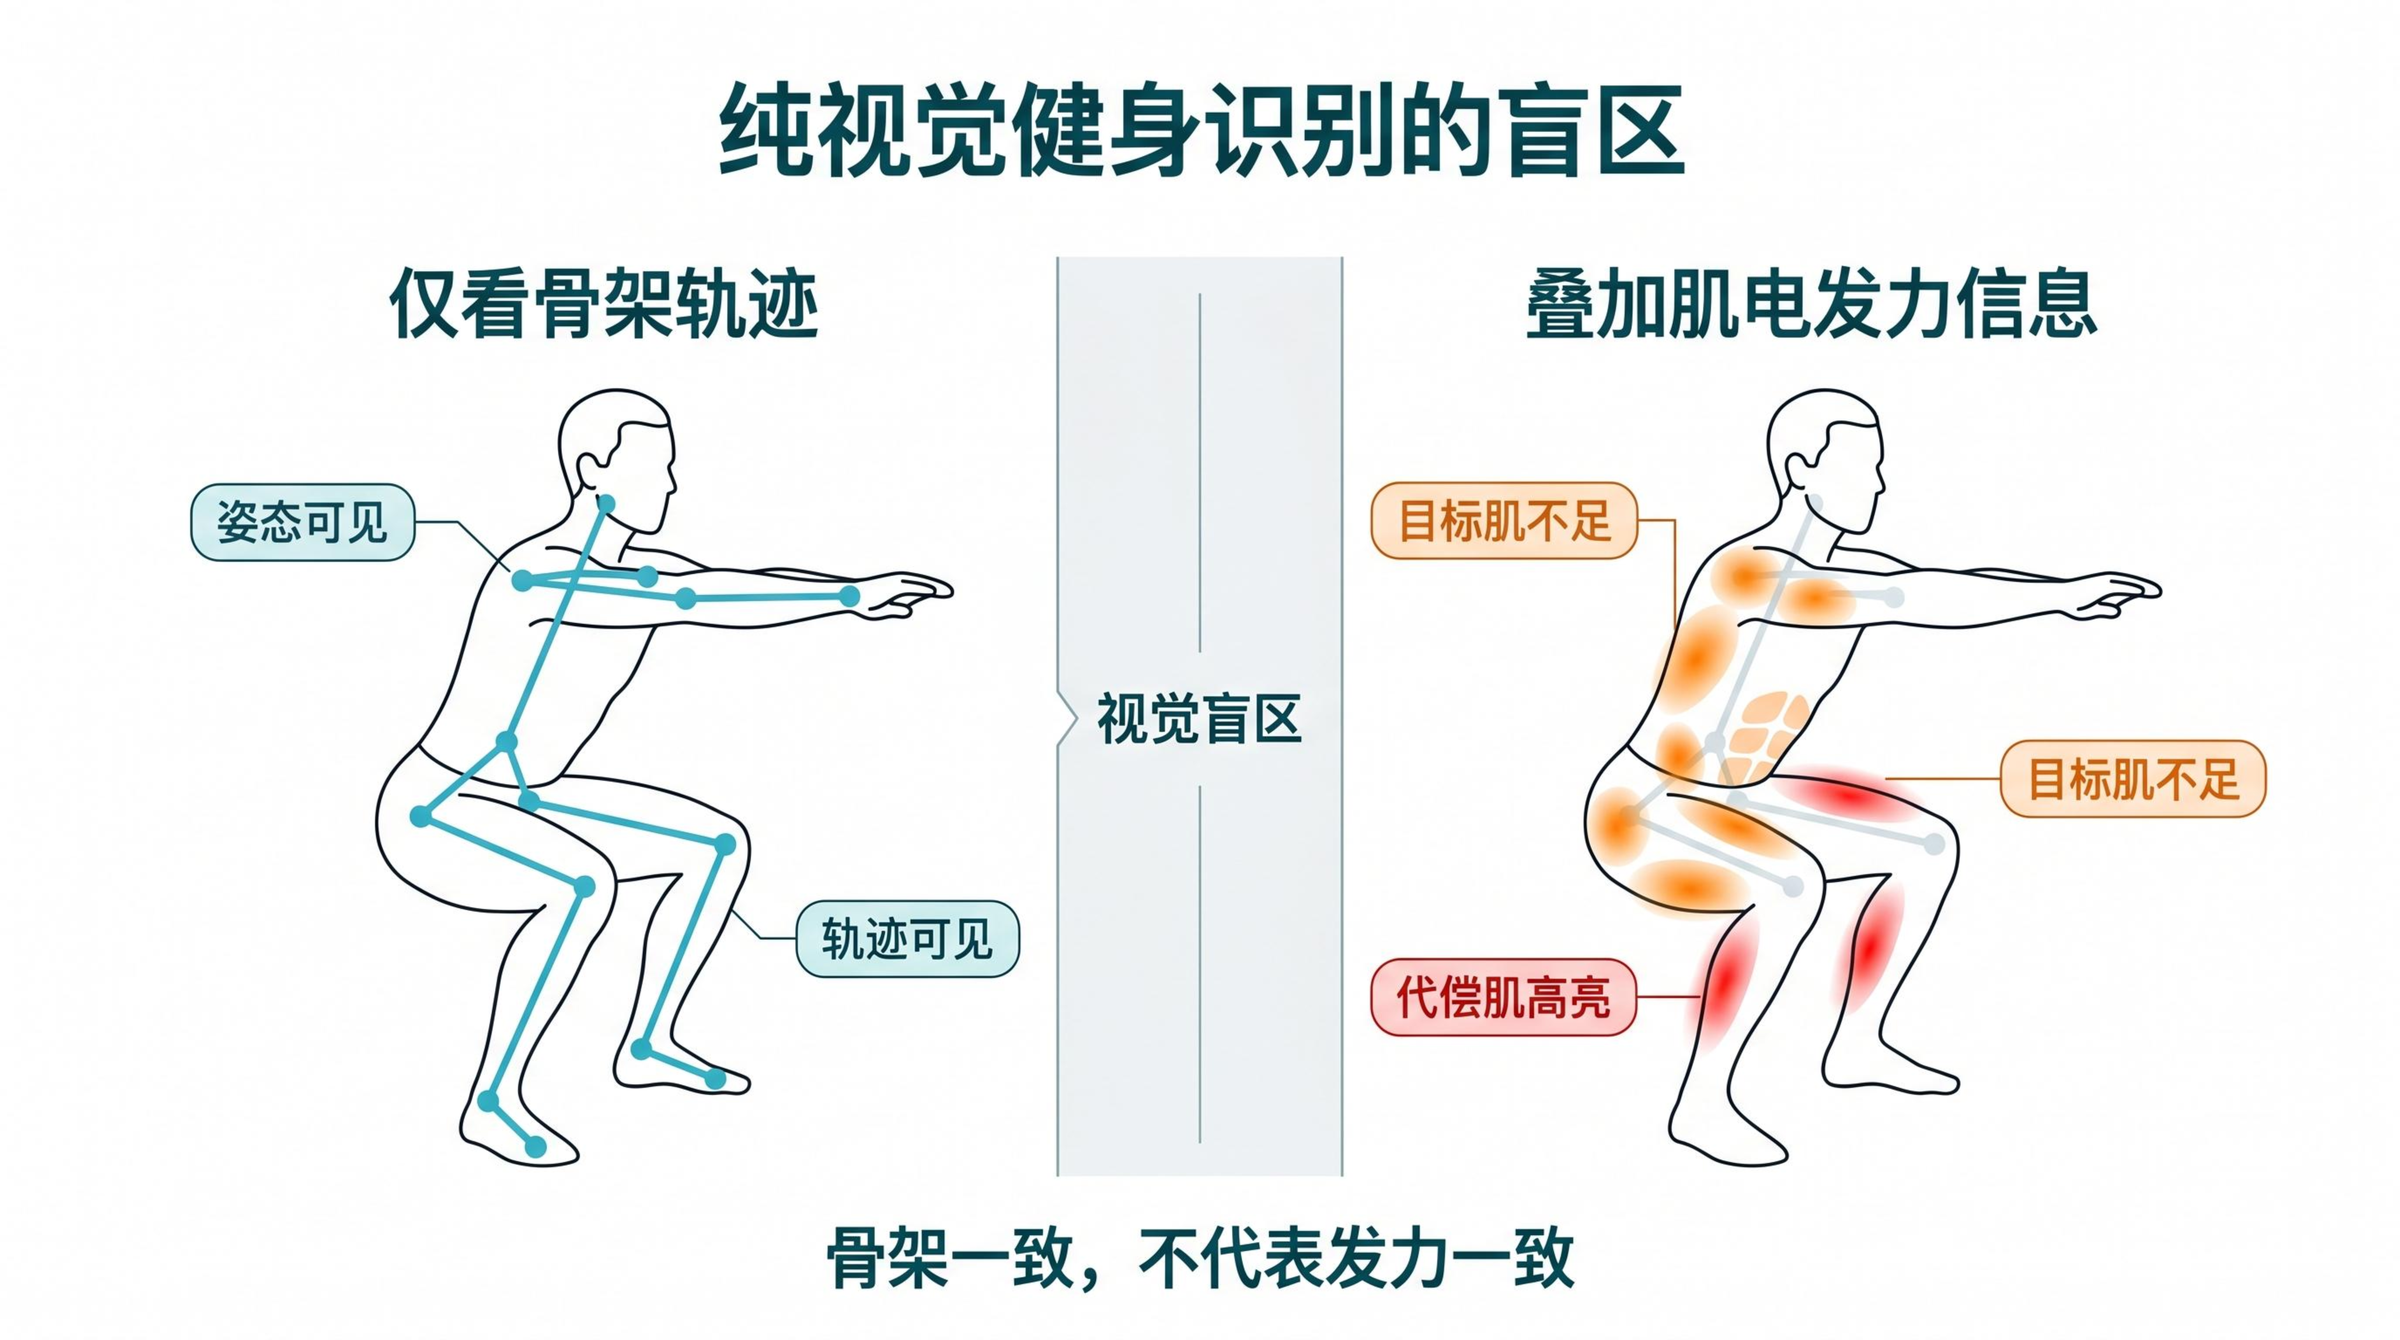
\includegraphics[width=0.88\textwidth]{figures/report/fig01.png}
    \caption{视觉姿态与肌电发力信息的互补关系示意。}
    \label{fig:vision-blind-spot}
\end{figure}

表面肌电（surface EMG, sEMG）提供了另一条观察路径。电极贴在皮肤表面
后，可以采集肌肉收缩时产生的微弱电信号。它不能替代视觉，因为肌电本身
不知道身体姿态；但它可以补上视觉看不到的肌肉激活信息。本项目的
核心想法就是把这两类信息放在一起：视觉负责看动作阶段和外部轨迹，肌电
负责看目标肌肉和代偿肌肉的实际参与程度。

\subsection{项目希望解决的三个问题}

围绕这个出发点，本项目最终要解决的不是单点算法问题，而是一条完整
的嵌入式系统链路。

\begin{enumerate}
    \item \term{感知问题}：如何同时拿到视觉姿态和肌电信号，并让它们在
    同一组动作里对齐。视觉帧率、肌电采样频率和动作周期都不一样，直接
    把原始数据拼在一起并不现实。

    \item \term{判断问题}：如何判断一次动作到底是标准、不标准，还是
    发生了代偿。这个判断不能只靠硬编码阈值，否则每换一个动作、一个人
    或一套贴片位置，都需要重新调参数。

    \item \term{交互问题}：用户运动时手上可能拿着哑铃，身上有汗，触屏
    操作并不方便。因此系统需要尽量用语音完成动作切换、训练反馈和简单
    对话，让前端更多承担展示而不是控制入口。
\end{enumerate}

这三个问题决定了项目的形态：它不是一个单独的识别模型，也不是一个只有
网页界面的健身小工具，而是一套由硬件、边缘计算、模型推理、语音交互和
本地前端共同组成的系统。

\subsection{设计目标与预期效果}

本项目的目标是设计一套面向个人训练场景的智能健身教练系统。它不只记录
用户做了多少次动作，还要尽量回答三个更接近训练结果的问题：动作过程是否
稳定，目标肌是否参与发力，是否出现明显代偿。为此，系统需要把视觉姿态、
肌电激活、动作阶段、语音交互和训练记录放入同一条链路中，让一次训练从
感知、判断到反馈都能被连续描述。

预期效果可以概括为四点。第一，用户穿戴贴片和腰包后，系统能够采集姿态和
肌电两类信号；第二，系统能够根据动作阶段、目标肌激活和代偿趋势给出
结果导向的训练反馈；第三，语音交互能够承担运动中的动作切换、参数调整和
训练总结，减少对触屏操作的依赖；第四，训练记录和后台调试信息能够沉淀
下来，为长期偏好、个性化校准和后续功能升级提供依据。

目前系统已经形成了上述目标的主体形态：RK3399ProX 负责边缘计算和本地
服务，ESP32 肌电单元负责无线传输，视觉和肌电共同进入 FSM/GRU 判断链路，
语音、Web 前端和数据库记录负责反馈与复盘。后续工作的重点不是改变这个
总体方向，而是继续提高真实佩戴、连续肌电输入和长期数据积累的稳定性。

\smallskip
\noindent\textbf{全文组织。} 第 \ref{sec:hardware} 章介绍硬件平台与无线
通信拓扑；第 \ref{sec:methodology} 章按"感知—判断—交互"三层组织
核心技术路线；第 \ref{sec:implementation} 章描述软件架构与主要模块
实现；第 \ref{sec:debug} 章复盘工程调试中影响系统形态的关键问题；
第 \ref{sec:conclusion} 章总结贡献、不足与后续方向。

\section{硬件生态与无线通信拓扑}
\label{sec:hardware}

\subsection{板端主机与外设}

本项目的板端主机使用 RK3399ProX 开发板。它承担本地服务、状态机、
Web 前端、语音守护进程和部分视觉推理任务，也是各类传感数据最终汇合的
节点。板端外设主要包括摄像头、麦克风、扬声器或外接音箱，以及 Web 网页
展示所需的网络入口。这样的组合优先保证多路输入能够稳定汇聚，并让
训练状态、传感状态和调试信息可以被直接观察。

\begin{figure}[htbp]
    \centering
    \includegraphics[width=0.92\textwidth]{figures/report/fig02-board.png}
    \caption{RK3399ProX 板端主机及外设连接实拍。}
    \label{fig:board-photo}
\end{figure}

摄像头负责提供视觉姿态估计输入，麦克风和扬声器负责语音交互，Web 前端
则承担训练状态、肌电波形、模式信息和调试入口的展示。把这些外设接到同一
板端后，系统不再是几个独立功能的拼接，而是可以围绕一次训练流程组织
输入、判断和反馈。

\subsection{ESP32 肌电传输单元}

肌电侧由贴片电极、肌电采集模块、ESP32 主控和电源组成。贴片电极贴在
目标肌和可能代偿的肌群附近，采集模块完成模拟前端处理，ESP32 负责读取
通道值并通过无线链路发送到板端。这个单元的设计重点是把采集、供电、
无线传输和佩戴固定组织成一条可连续工作的传感链路。

\begin{figure}[htbp]
    \centering
    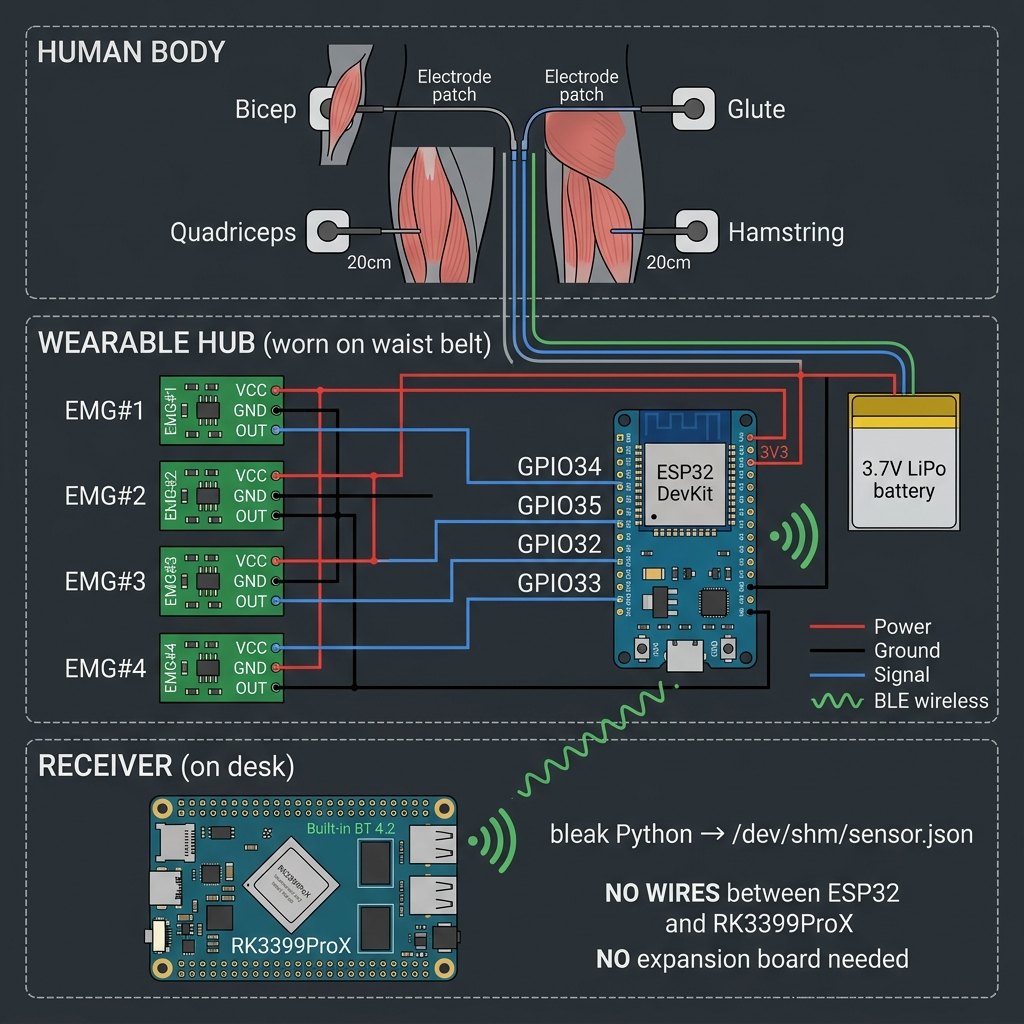
\includegraphics[width=0.72\textwidth]{figures/report/fig03-unit.jpg}
    \caption{肌电采集与传输单元早期结构示意。}
    \label{fig:wearable-concept}
\end{figure}

肌电信号幅值很小，对接地、布线和贴片稳定性都比较敏感。项目后期的方向是
把采集板、ESP32 主控和电源进一步集中到一块自制集成板中，再通过更短的
线路引出到目标肌群。这样做有三个好处：装配时少接线、运动时线束更短、
电源和信号路径更容易固定。对可穿戴设备来说，这不仅是美观问题，也关系到
佩戴安全和信号稳定。

\subsection{穿戴结构与走线}

硬件佩戴方式同样影响系统可用性。最直接的做法是把板子和电极都固定在手臂
或腿上，但实际运动时会遇到两个问题：一是线束容易随动作摆动，二是贴片
受到拉扯后会改变接触状态。项目最终采用更稳妥的穿戴思路：主机、电池和
ESP32 放在腰包或贴身固定区域，贴片只通过短线连接到目标肌群；运动服和
肩带用于固定线路，让设备不影响深蹲、弯举等动作。

\begin{figure}[htbp]
    \centering
    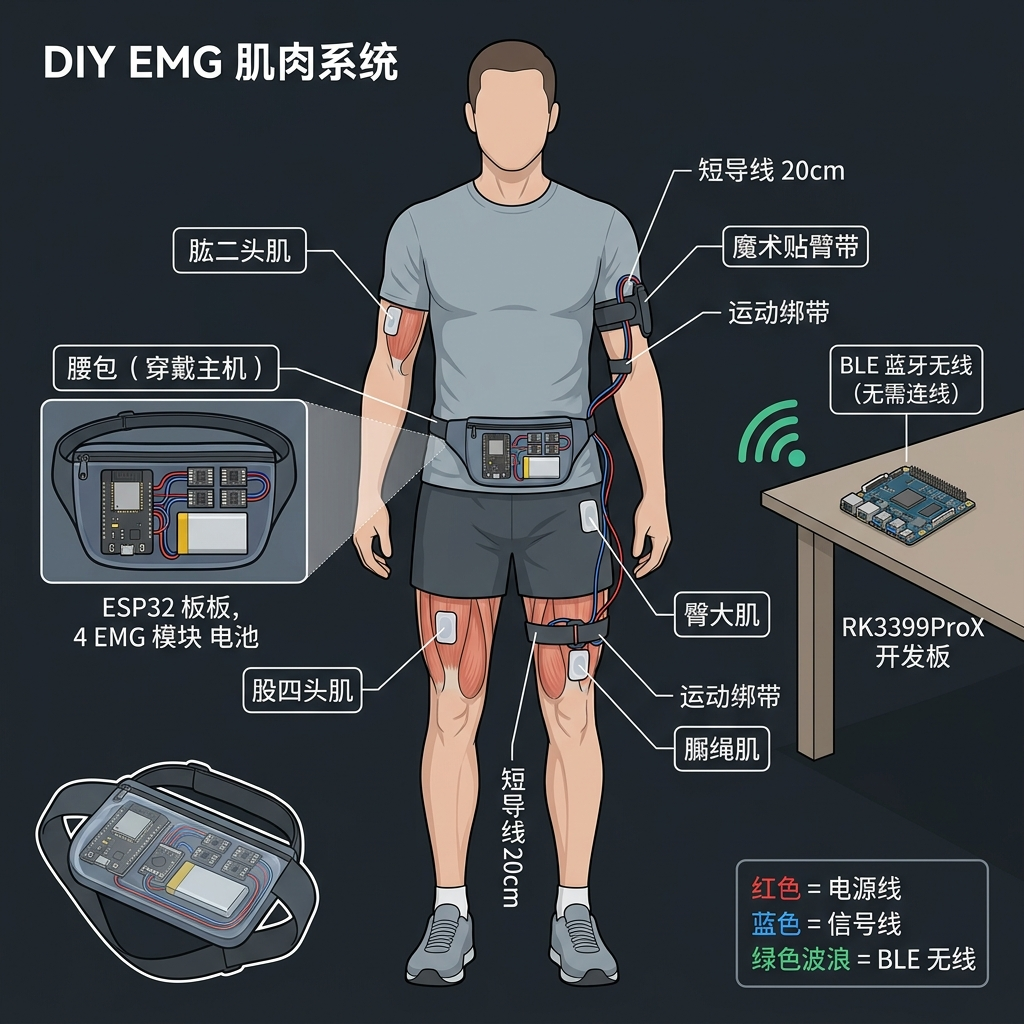
\includegraphics[width=0.85\textwidth]{figures/report/fig03-system.jpg}
    \caption{DIY 肌电系统整体穿戴示意：腰包集中放置 ESP32 主控、4 路 sEMG 采集模块和电池，贴片经短导线连接目标肌群，BLE/Wi-Fi 上行至 RK3399ProX 板端。}
    \label{fig:wearable-routing}
\end{figure}

这种结构的优点是把重量放在身体更稳定的位置，同时把敏感的电极线尽量贴近
身体走线。它还方便调试：需要更换贴片位置时，不必重新拆整套主机；需要
观察板端状态时，也可以直接从腰包或工作台取出模块。相比把多个模块分散
固定在四肢上，腰包和短线结构更容易控制重量分布和线束拉扯。

\subsection{从 BLE 到 Wi-Fi UDP}

无线通信路线保留了项目里的一个真实转折。早期使用 BLE，是因为它低功耗、
资料多，也符合可穿戴设备的常见直觉。但肌电信号不是偶尔上报一次的状态量，
而是连续变化的时序数据。通道数和采样频率提高以后，BLE 的连接间隔、握手
和吞吐限制逐渐影响连续数据流。

项目最终改用 Wi-Fi UDP。ESP32 不再维护复杂连接状态，而是把每帧肌电特征
封装成 UDP 数据报发给 RK3399ProX。UDP 没有重传和确认机制，表面上不如
可靠传输完整；但对于滑动窗口和动作周期分析来说，偶尔丢失一个瞬时点通常
比整条反馈链路持续堆积延迟更容易处理。健身反馈更需要连续、轻量、能容忍偶发丢点
的数据流，而不是把所有历史包都排队补齐。

\begin{figure}[htbp]
    \centering
    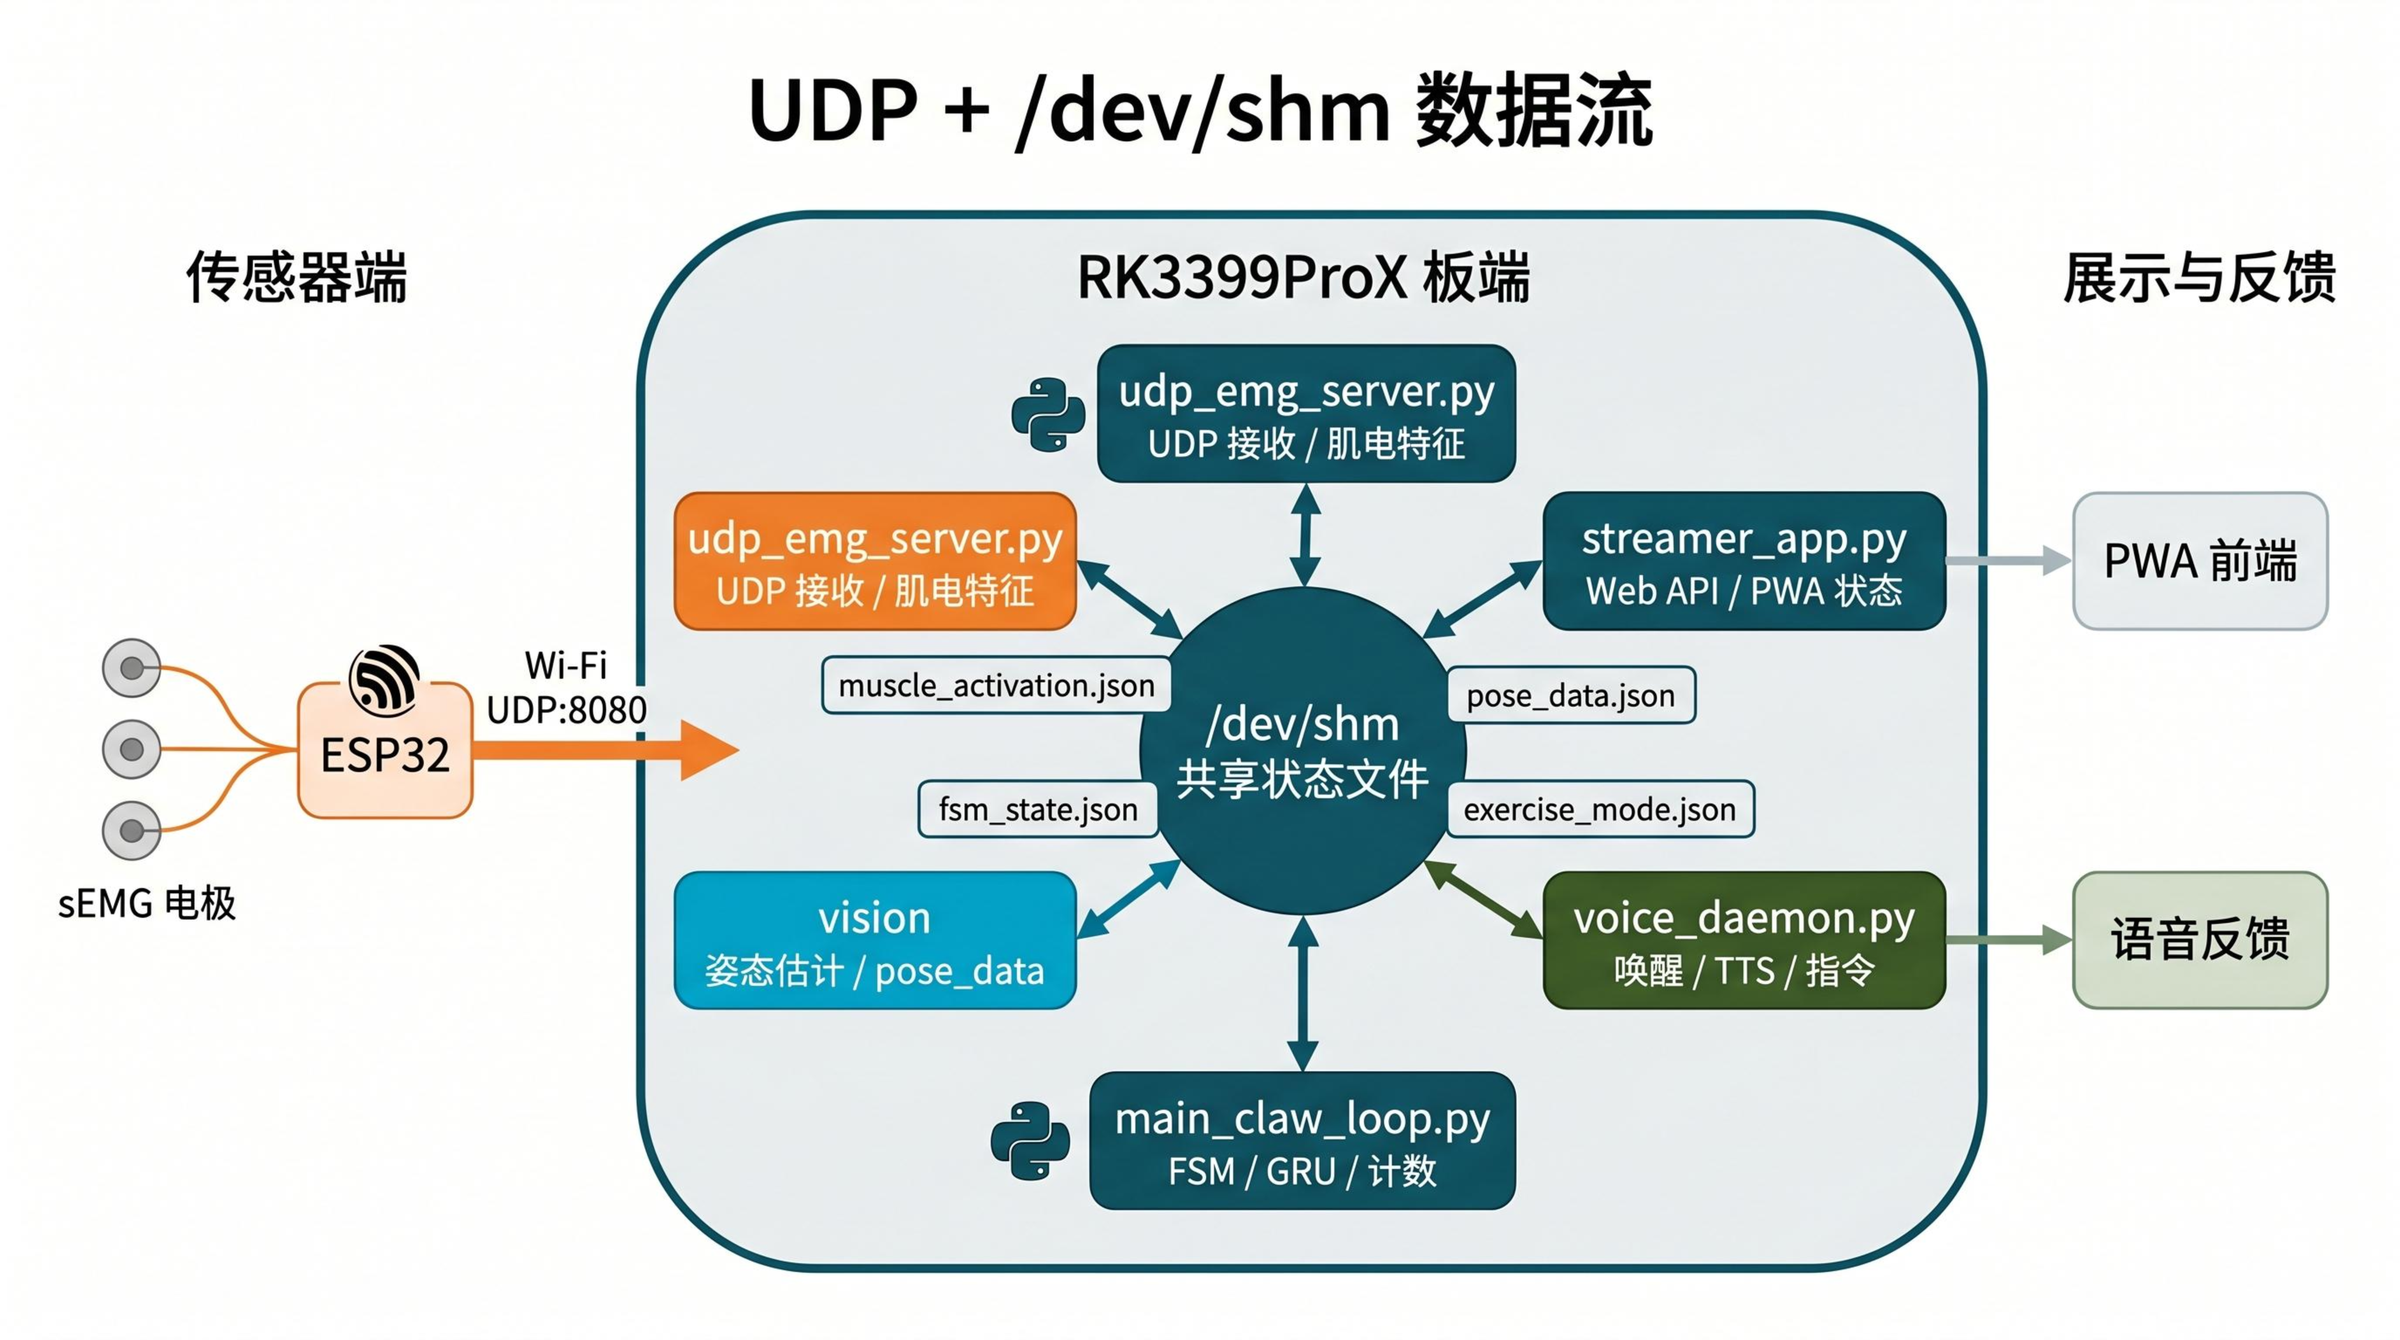
\includegraphics[width=0.92\textwidth]{figures/report/fig04.png}
    \caption{肌电数据从 ESP32 进入板端后的通信与共享状态文件流向。}
    \label{fig:udp-shm-dataflow}
\end{figure}

\subsection{硬件结构与集成方向}

采集板的原理图和 PCB 布局反映了接口、电源、固定孔和模拟/数字区域的
基本关系。完整电路细节以源文件为准，正文主要关注采集、传输和佩戴结构
之间的系统关系。

\begin{figure}[htbp]
    \centering
    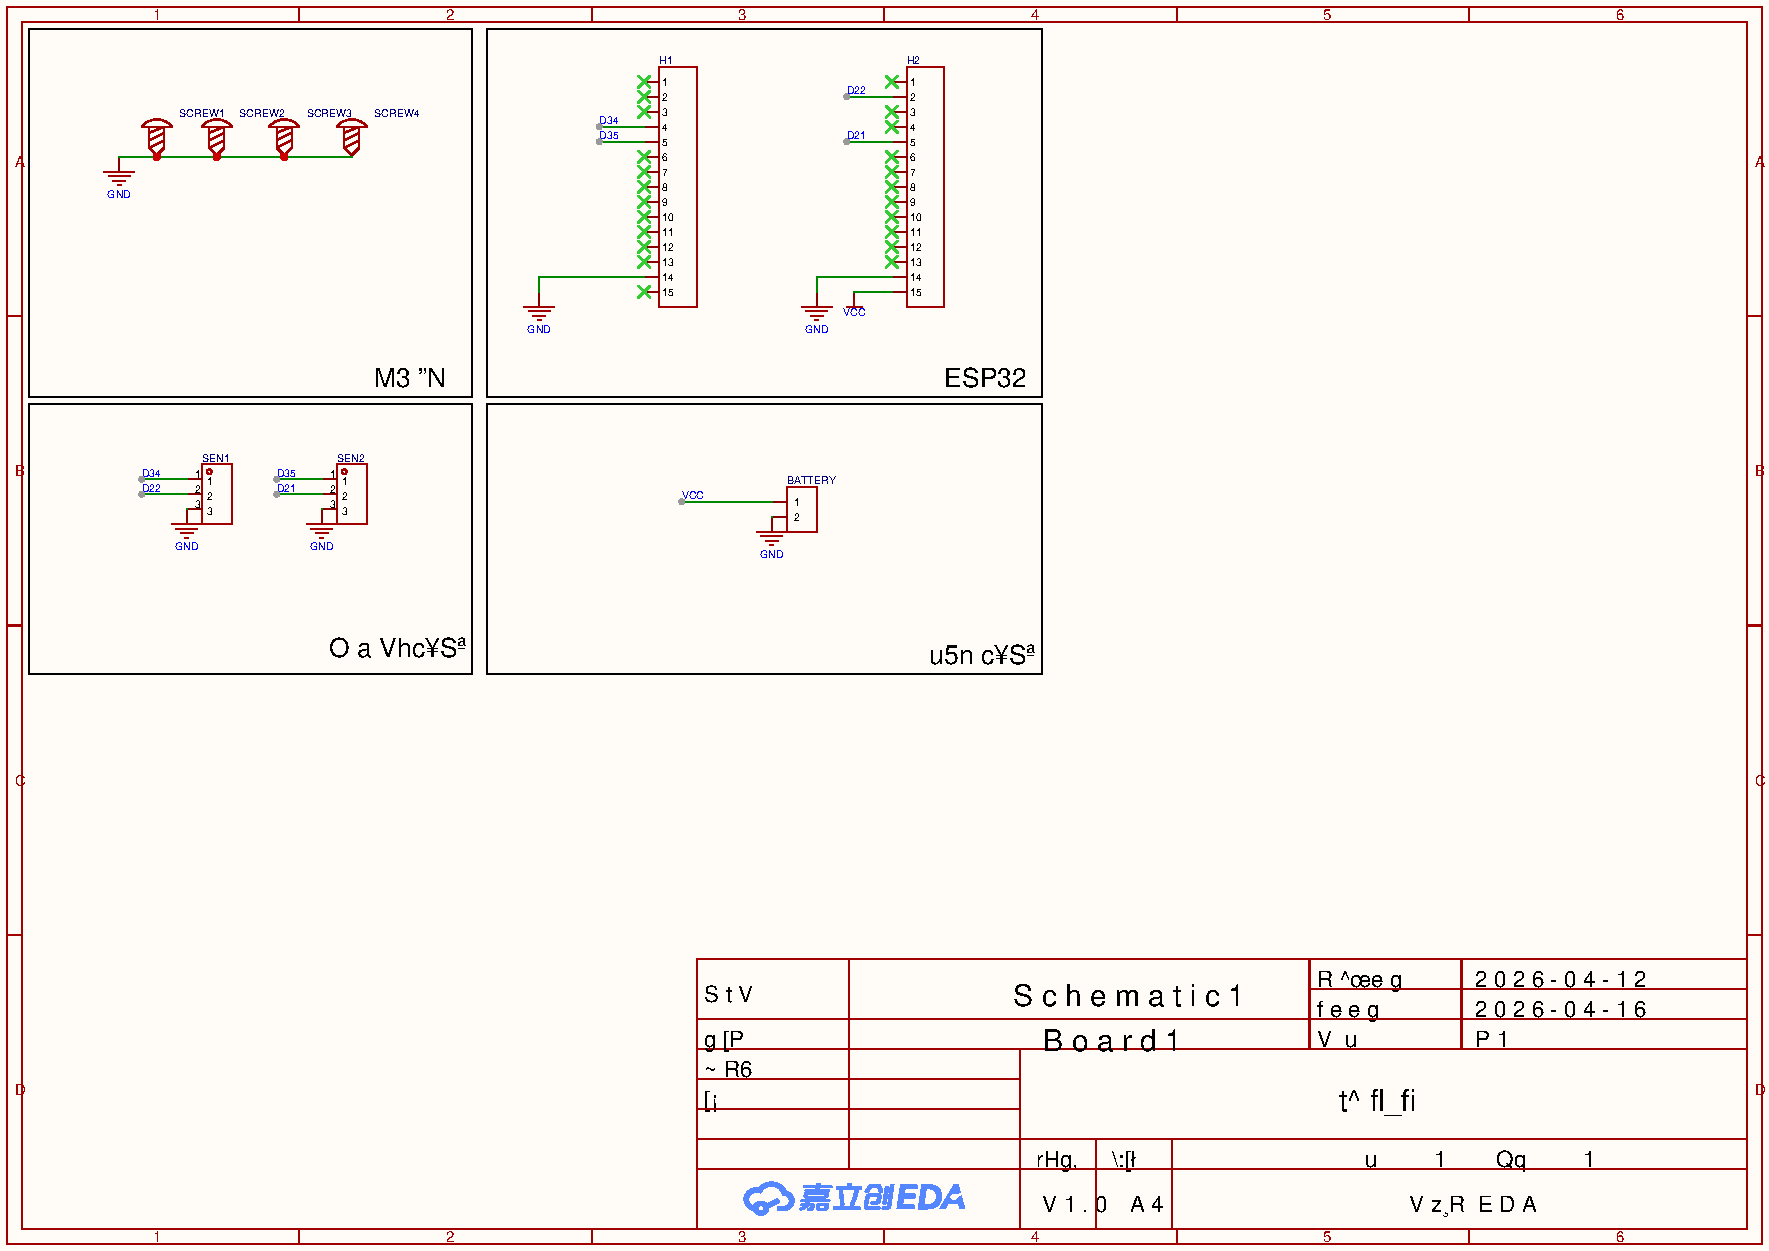
\includegraphics[width=0.94\textwidth]{figures/report/hw01.pdf}
    \caption{肌电采集板原理图概览。}
    \label{fig:hardware-schematic}
\end{figure}

\begin{figure}[htbp]
    \centering
    \includegraphics[page=4,width=0.42\textwidth]{figures/report/hw02.pdf}
    \caption{肌电采集板 PCB 局部布局。}
    \label{fig:hardware-pcb}
\end{figure}


\section{核心技术路线与关键决策}
\label{sec:methodology}

本项目的技术路线最终收敛为一条比较清楚的主线：视觉负责动作阶段和
外部姿态，肌电负责目标肌和代偿肌的激活变化，FSM 负责确定性计数，
CompensationGRU 负责一段动作窗口内的质量判断，DeepSeek 和后台记录接口
负责交互与长期材料沉淀。本章按"感知—判断—交互"三层组织：先讲系统
怎么拿到稳定的视觉姿态与肌电特征，再讲怎么把它们转化为可判断的动作
质量，最后讲判断结果如何变成用户能感知、系统能记住的反馈。

\subsection{感知层：拿到能用的姿态与肌电}

本节说明系统如何同时拿到稳定的视觉姿态与肌电信号，以及为什么把视觉做成
本地与云端双路、把肌电做 MVC 归一化。

\subsubsection{视觉双路：本地 NPU 与云端 RTMPose}

视觉模块保留两条路线：本地 YOLOv5-Pose RKNN 路线和云端 RTMPose 路线。
YOLOv5 是 Ultralytics 维护的单阶段目标检测模型 \cite{yolov5}；
YOLOv5-Pose 由 Maji 等人在 YOLO-Pose 工作中提出，把人体关键点回归与
目标检测做成端到端单阶段输出 \cite{yolopose2022}，便于转换为 RKNN
后在 RK3399ProX 的 NPU 上运行。本地路线的意义是让系统在网络条件变化
时仍能获得骨架关键点，并把关节角度和动作阶段持续送入后续状态机。

RTMPose 是 OpenMMLab 团队提出、在 MMPose 工具箱中开源的实时人体姿态
估计模型 \cite{rtmpose,mmpose}。与 YOLOv5-Pose 的端到端单阶段不同，
RTMPose 走自顶向下的两阶段路线（先检测人体框，再回归关键点），
关键点精度通常更高但计算量更大，因此在系统中作为云端 GPU 备选路线：
板端把摄像头帧发到云端服务，云端返回关键点 JSON，板端再把结果写入
统一姿态状态。

两条路线通过 \code{/dev/shm/vision_mode.json} 切换，最终都输出到统一的
姿态数据接口。这样的设计不是简单堆叠模型，而是保留探索空间：本地 NPU
路线关注低依赖运行，云端 RTMPose 路线关注关键点质量，两者服务于同一套
FSM、GRU 和训练反馈链路。

\begin{figure}[htbp]
    \centering
    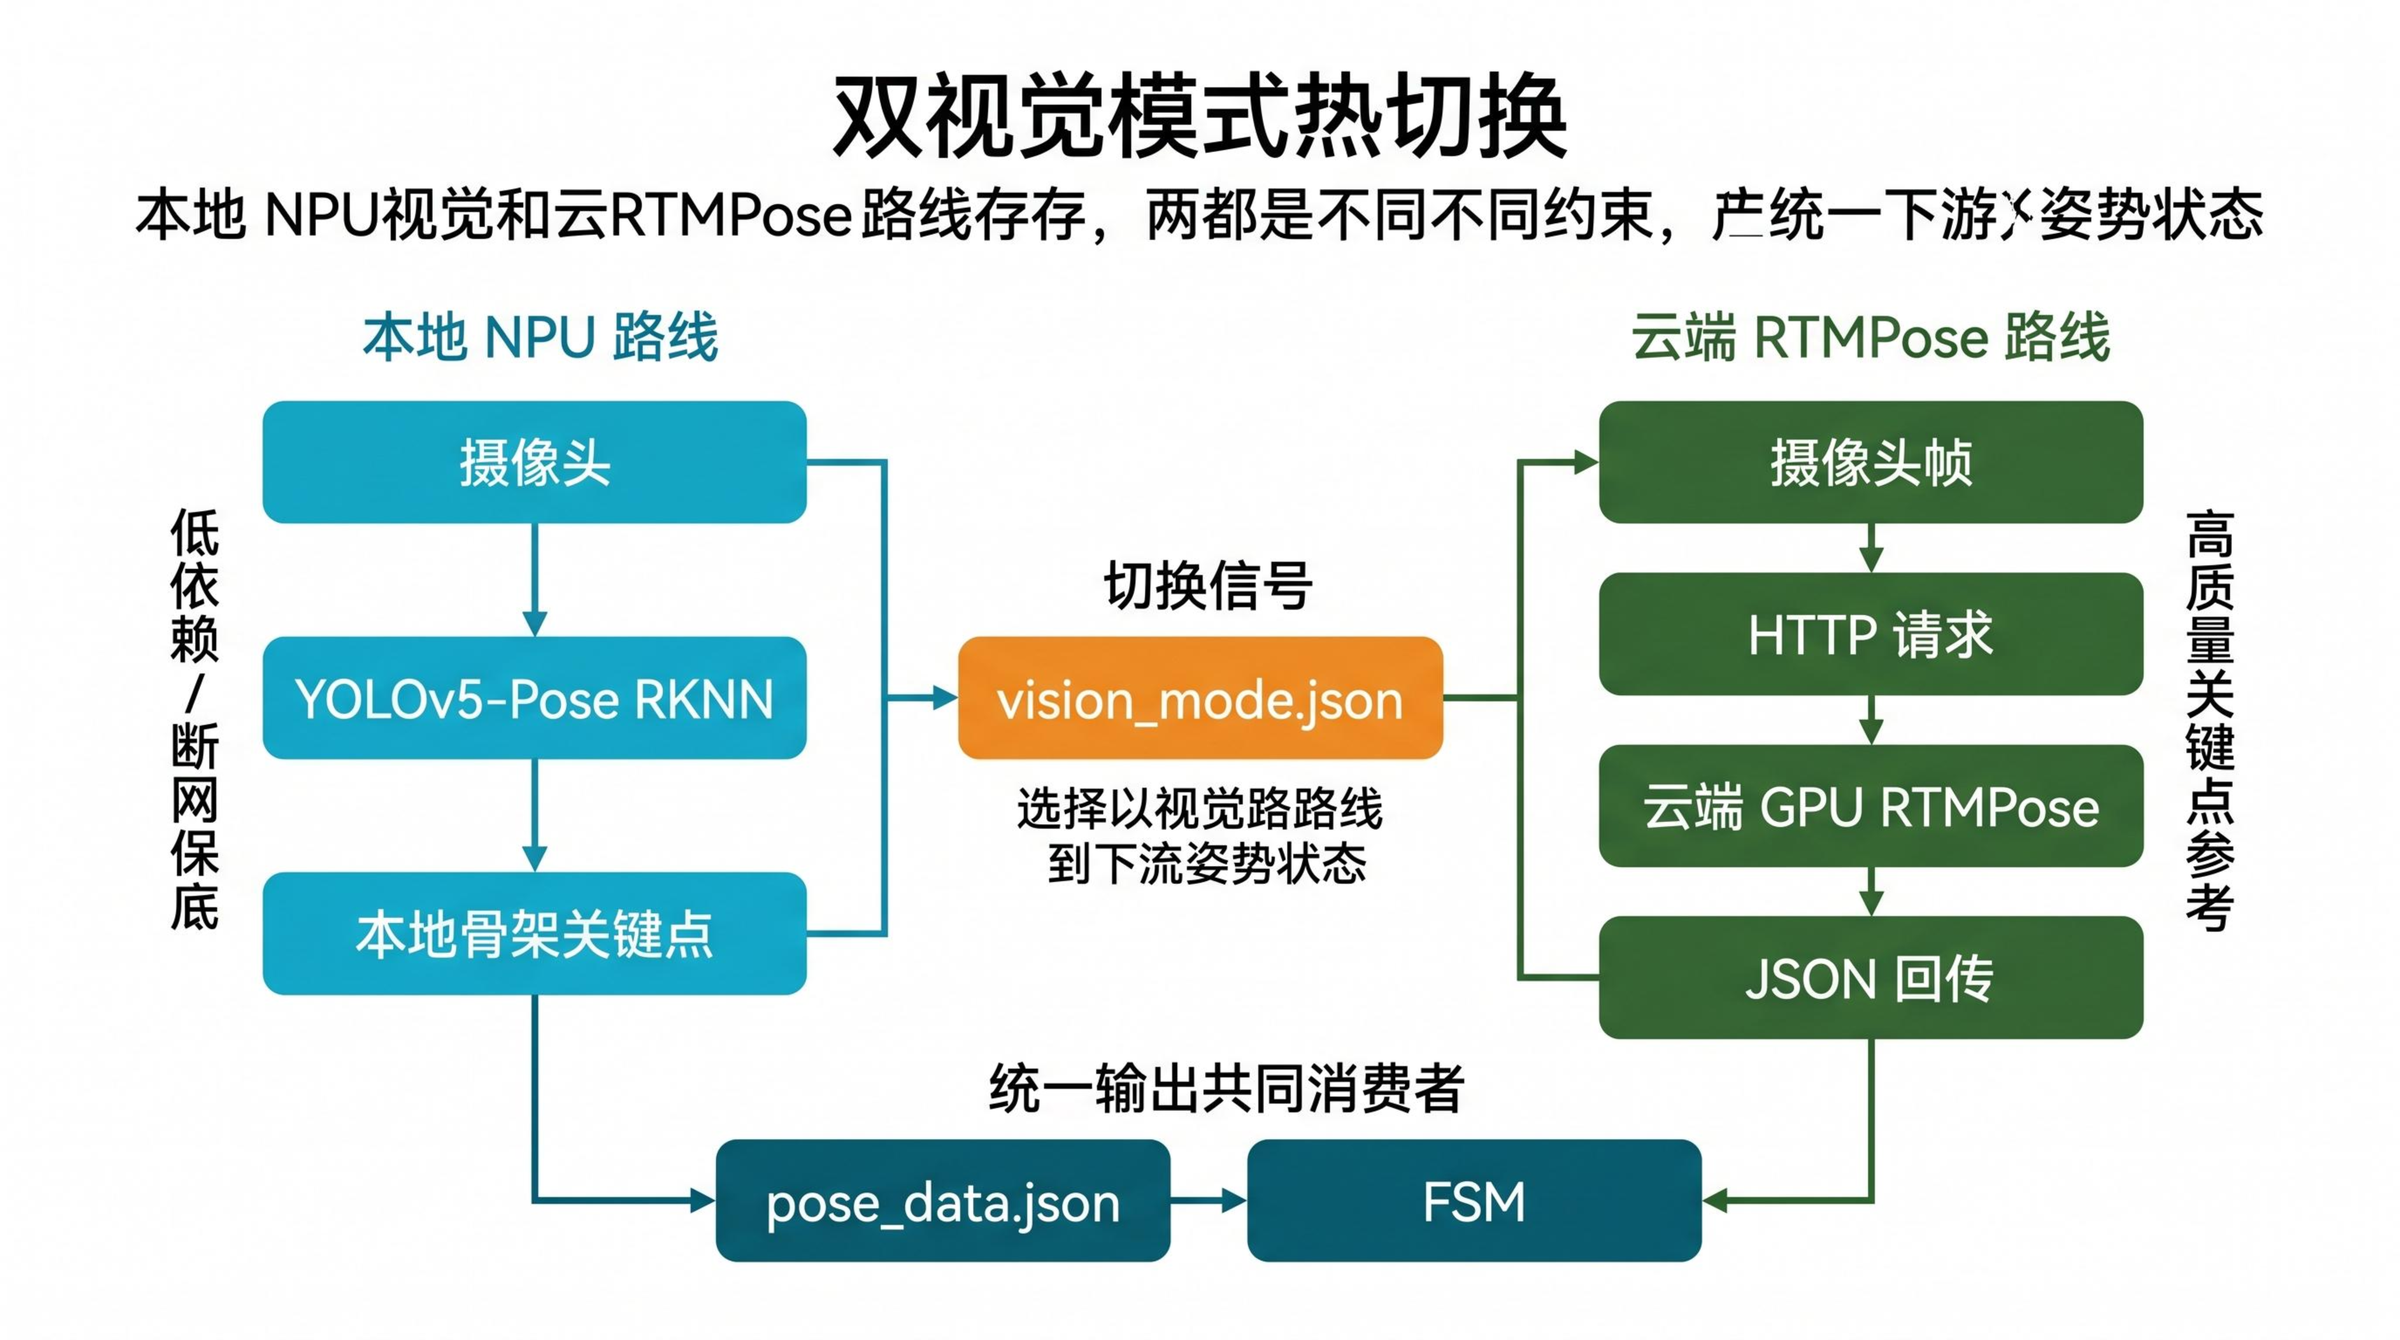
\includegraphics[width=0.92\textwidth]{figures/report/fig08.png}
    \caption{本地 NPU 与云端 RTMPose 并存的视觉路线。}
    \label{fig:dual-vision-switch}
\end{figure}

\subsubsection{肌电特征：MVC 归一化与个性化基准}

肌电特征不能直接用固定硬阈值解释。表面肌电的幅值会受到电极位置、皮肤
状态、个体肌肉基础、阻抗和动作方式影响。SENIAM 对表面肌电采集和电极
放置提出了规范建议 \cite{seniam}，EMG 幅值归一化也被长期讨论
\cite{burden2010,cede2020}。项目采用 MVC（Maximum Voluntary
Contraction）思路，让用户在训练前进行短时间最大发力，把该用户的峰值
作为个人基准。

在系统中，原始 RMS 经过个人 MVIC 峰值归一化后再进入特征窗口：
\[
    \%\mathrm{MVC}(t) = \frac{\mathrm{RMS}(t)}{\mathrm{MVIC}_{\mathrm{peak}}}\times 100\%.
\]
这是肌电幅值归一化的常见表达 \cite{burden2010,cede2020}。该数值不等于
严格的机械做功，更适合作为目标肌相对发力水平的工程近似。这样做的意义
在于，同一个固定阈值不会直接套在所有人身上，模型看到的是更接近"相对
发力水平"的输入。

\begin{figure}[htbp]
    \centering
    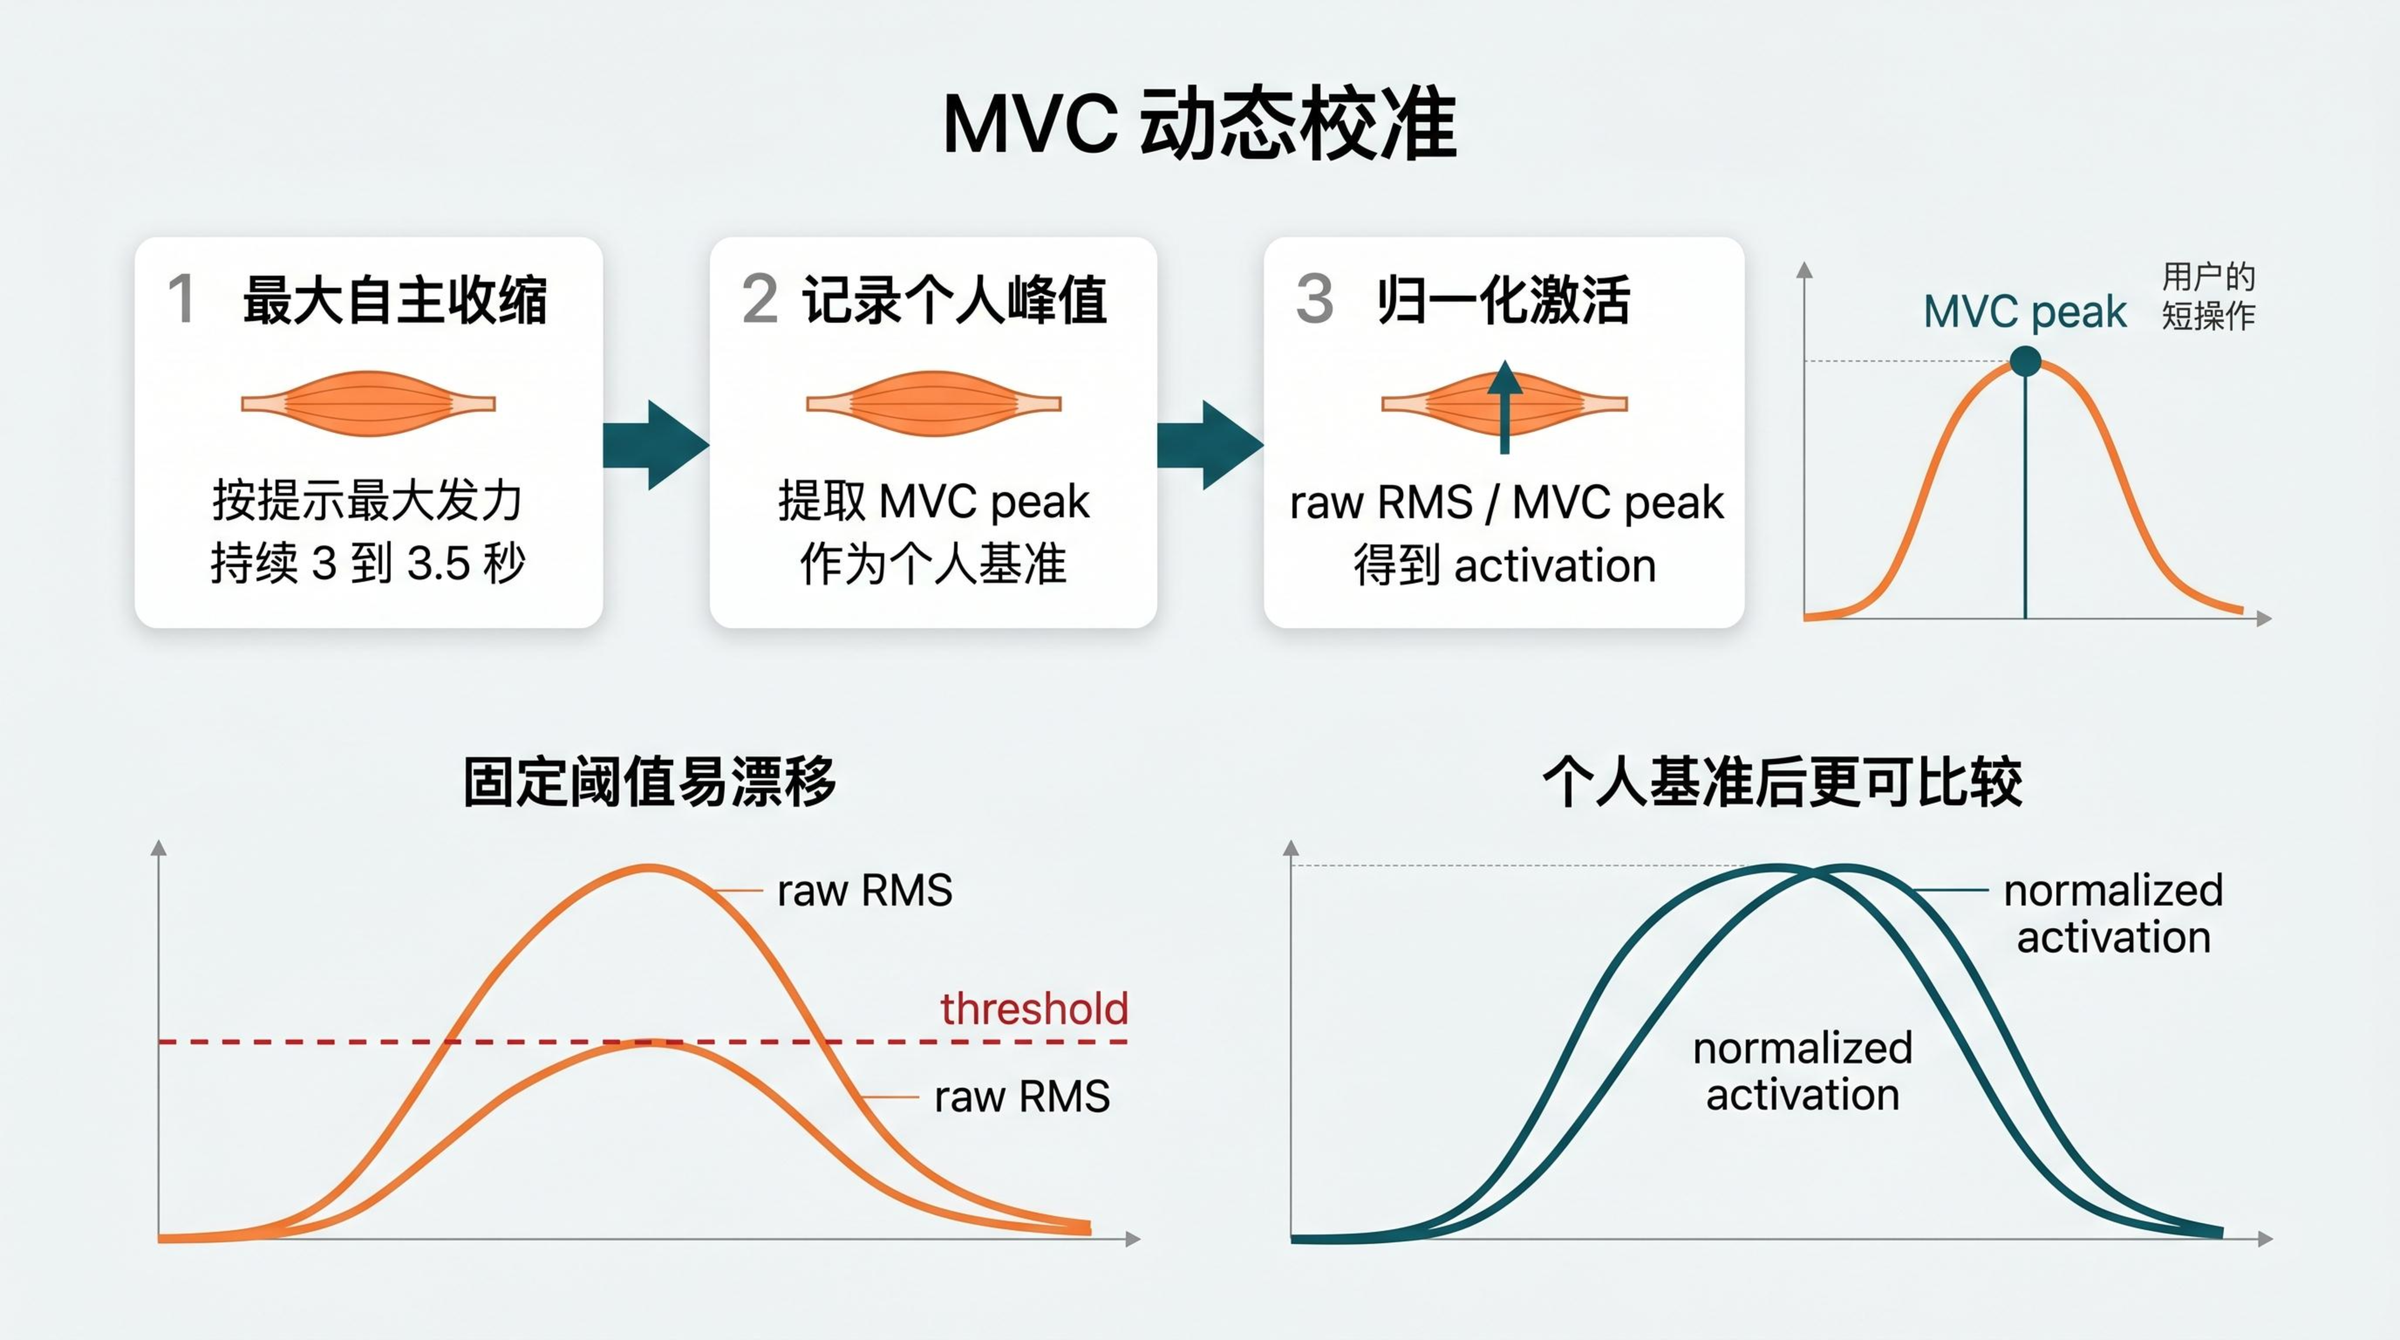
\includegraphics[width=0.9\textwidth]{figures/report/fig07.png}
    \caption{MVC 归一化校准流程示意。}
    \label{fig:mvc-calibration}
\end{figure}

\subsection{判断层：FSM 与 GRU 的分工}

感知层提供原始信号后，下一步要把它转化为可判断的动作质量。本节讨论
FSM 与 GRU 的分工，以及为什么选择 Mid-Fusion 而非端到端融合。

\subsubsection{从 if/else 到 GRU}

动作判断最终采用 FSM 与 GRU 分工，而不是只用规则或只用神经网络。FSM
负责动作阶段、上下行切换和次数统计，因为这部分与关节角度变化直接相关，
规则清楚、响应快，也方便调试。GRU 负责动作质量分类，因为代偿不是一个
单点阈值，而是一段动作周期里目标肌、代偿肌和动作相位之间的关系。

早期的 if/else 规则有明显优势：容易解释、容易快速跑通，也方便确认角度
阈值是否合理。但继续扩展到肌电后，规则很快变得脆弱。不同人、不同贴片
位置、不同动作幅度都会改变 RMS 分布；代偿动作也不一定表现为某一帧
突然越过阈值。门控循环单元（GRU）最早出现在 Cho 等人 2014 年提出的
RNN encoder-decoder 框架 \cite{gru} 中，它通过更新门与重置门在保留
历史状态和接收当前输入之间取得平衡，比朴素 RNN 更适合处理有限窗口
内的时序变化。本项目把最近一段 7D 特征窗口交给 CompensationGRU 做
标准、代偿和不标准三类判断。

\subsubsection{Mid-Fusion：在特征层融合}

多模态融合最终采用 Mid-Fusion \cite{baltrusaitis2018}。也就是说，视觉
和肌电不直接把原始序列硬拼进一个大模型，而是先转成低维、可解释的特征，
再进入轻量时序模型。视觉侧提取关节角度、角速度、角加速度和动作相位；
肌电侧提取目标肌 RMS、代偿肌 RMS，并结合对称性或阶段信息形成 7D 特征。
这个设计让模型输入更稳定，也让调试时能看懂每一列数据代表什么。

端到端融合在概念上更完整，但并不适合本项目当前条件。视觉关键点是低频
几何序列，肌电是更高频的生理信号；直接拼接会把时间对齐和噪声处理都推给
模型。板端算力、数据规模和现场调试也不支持一开始就采用复杂融合网络。
Mid-Fusion 把领域知识放在特征层，既保留了视觉和肌电的互补关系，也把
模型复杂度控制在当前板端和数据规模能够承受的范围内。

\begin{figure}[htbp]
    \centering
    \resizebox{0.96\textwidth}{!}{%
    \begin{tikzpicture}[
        node distance=0.9cm and 1.0cm,
        box/.style={draw, rounded corners=2pt, align=center, minimum width=2.8cm,
                    minimum height=0.8cm, font=\small},
        vision/.style={box, fill=cyan!9, draw=cyan!60!black},
        emg/.style={box, fill=orange!12, draw=orange!75!black},
        fuse/.style={box, fill=teal!10, draw=teal!70!black, minimum width=3.0cm},
        model/.style={box, fill=green!9, draw=green!55!black, minimum width=2.9cm},
        classout/.style={box, fill=gray!7, draw=gray!65, minimum width=1.7cm},
        arrow/.style={-{Latex[length=2mm]}, thick}
    ]
        \node[vision] (camera) {摄像头\\骨架关键点};
        \node[vision, right=of camera] (vfeat) {视觉特征\\关节角 / 角速度 / 相位};
        \node[emg, below=1.2cm of camera] (sensor) {sEMG 电极\\ESP32 UDP};
        \node[emg, right=of sensor] (efeat) {肌电特征\\RMS / MVC 归一化};
        \node[fuse, right=1.2cm of vfeat, yshift=-0.6cm] (window)
            {7D 特征窗口\\角度、角速度、角加速度\\目标肌 RMS、代偿肌 RMS\\对称性、动作相位};
        \node[model, right=1.0cm of window] (gru) {CompensationGRU\\轻量时序判断};
        \node[classout, right=0.9cm of gru, yshift=0.78cm, fill=green!12] (std) {标准};
        \node[classout, right=0.9cm of gru, fill=orange!12, draw=orange!70!black] (comp) {代偿};
        \node[classout, right=0.9cm of gru, yshift=-0.78cm, fill=red!8, draw=red!55!black] (bad) {不标准};

        \node[font=\bfseries\small, above=0.18cm of camera] {视觉流};
        \node[font=\bfseries\small, below=0.18cm of sensor] {肌电流};
        \node[font=\bfseries\small, above=0.18cm of window] {特征融合};
        \node[font=\bfseries\small, above=0.18cm of gru] {时序分类};

        \draw[arrow, cyan!70!black] (camera) -- (vfeat);
        \draw[arrow, orange!80!black] (sensor) -- (efeat);
        \draw[arrow, cyan!70!black] (vfeat) -- (window);
        \draw[arrow, orange!80!black] (efeat) -- (window);
        \draw[arrow, teal!75!black] (window) -- (gru);
        \draw[arrow, green!55!black] (gru) -- (std);
        \draw[arrow, orange!75!black] (gru) -- (comp);
        \draw[arrow, red!55!black] (gru) -- (bad);
    \end{tikzpicture}}
    \caption{Mid-Fusion 多模态特征融合路线。}
    \label{fig:mid-fusion}
\end{figure}

\subsection{交互层：LLM 与后台记录的边界}

判断结果最终要变成用户能看懂、系统能记住的反馈。本节说明 LLM 在前台
对话与后台总结之间的分工，以及训练数据的来源与边界。

\subsubsection{LLM 实时对话与后台总结分工}

大语言模型在系统里承担两类时间尺度不同的任务。前台 DeepSeek 主要用于
语音问答、训练提示和总结生成，要求上下文短、响应快；后台记录、数据库
和 OpenClaw 相关接口更适合保存训练历史、偏好变化和周期性总结，允许
更长的上下文和更慢的处理。项目把二者分开，是为了避免实时反馈被长期
分析拖慢，也避免后台记录直接影响训练主链路。

当前系统已经能展示知识库命中、云端记忆、数据库表和调试入口。它们的
价值在于让训练数据和调试证据不再散落在黑盒里。长期记忆、用户画像和
周期性计划属于后续扩展方向；在当前报告中，它们作为可维护性和可演进性
的接口来描述。

\subsubsection{数据来源与训练边界}

多模态健身数据集是项目中的现实难点。公开数据可以提供动作周期、肌电
模式和姿态估计的先验，但很难完全匹配本项目的硬件、贴片位置、动作定义
和训练场景。项目因此采用公开数据、本地采集、模拟数据和数据增强结合
的路线：公开数据中，EMAHA-DB6 提供较完整的多通道 sEMG 动作样本，
MIA 数据集提供肌电与运动学同步标注，Mendeley 公开的 sEMG 弯举数据集
提供个体差异的参考分布；这些公开样本主要用于建立特征分布的先验，本地
采集用于贴近本项目的 ESP32 + 4 通道贴片硬件域，增强数据则在公开与
本地样本上进一步扩大训练过程中的扰动范围（噪声注入、随机平移、贴片
偏移模拟等）\cite{lara2013}。

增强数据和本地数据可以帮助模型学习当前任务中的区分信号，但训练策略
仅在当前数据规模下适用，不直接外推到跨用户、跨环境的稳定泛化。

\subsection*{本章小结}
\addcontentsline{toc}{subsection}{本章小结}

上述选择共同服务于一个目标：让系统在边缘设备上可运行、可调试，并能
围绕真实训练流程持续扩展。它们不是单点技术堆叠，而是围绕真实训练
流程不断收敛出来的工程取舍。

\begin{table}[htbp]
\centering
\small
\begin{tabular}{@{}>{\raggedright\arraybackslash}p{0.23\textwidth}
                >{\raggedright\arraybackslash}p{0.28\textwidth}
                >{\raggedright\arraybackslash}p{0.37\textwidth}@{}}
\toprule
\textbf{岔路} & \textbf{最后选择} & \textbf{原因} \\
\midrule
视觉模型 & YOLOv5-Pose + RTMPose 双路线 & 本地路线降低网络依赖，云端路线
提供关键点质量参考，通过状态文件切换。 \\
动作判断 & FSM 计数 + GRU 分类 & 计数是几何问题，质量判断是时序和肌电
共同作用的问题。 \\
多模态融合 & Mid-Fusion & 端到端融合对板端算力和数据规模要求过高，
先降维到可解释特征更稳。 \\
肌电基准 & MVC 归一化 & 用个人峰值减少固定阈值在不同个体之间的漂移。 \\
LLM 接入 & 实时对话 + 后台记录接口 & 即时反馈和长期整理的时间尺度不同，
拆开后边界更清楚。 \\
\bottomrule
\end{tabular}
\caption{项目中的关键技术取舍}
\label{tab:decisions}
\end{table}

\section{系统功能与软件架构}
\label{sec:implementation}

本章把 IronBuddy 的软件层拆成总体架构、训练业务和交互维护三层：4.1
说明系统如何用多进程和共享状态把视觉、肌电、语音、前端与后台记录隔离
开；4.2 在该骨架上描述训练业务如何从单纯计数推进到兼顾目标肌激活与
代偿判断；4.3 说明语音状态机、调试控制台和本地数据库如何让系统在功能
持续扩展时仍可复测。

\begin{figure}[htbp]
    \centering
    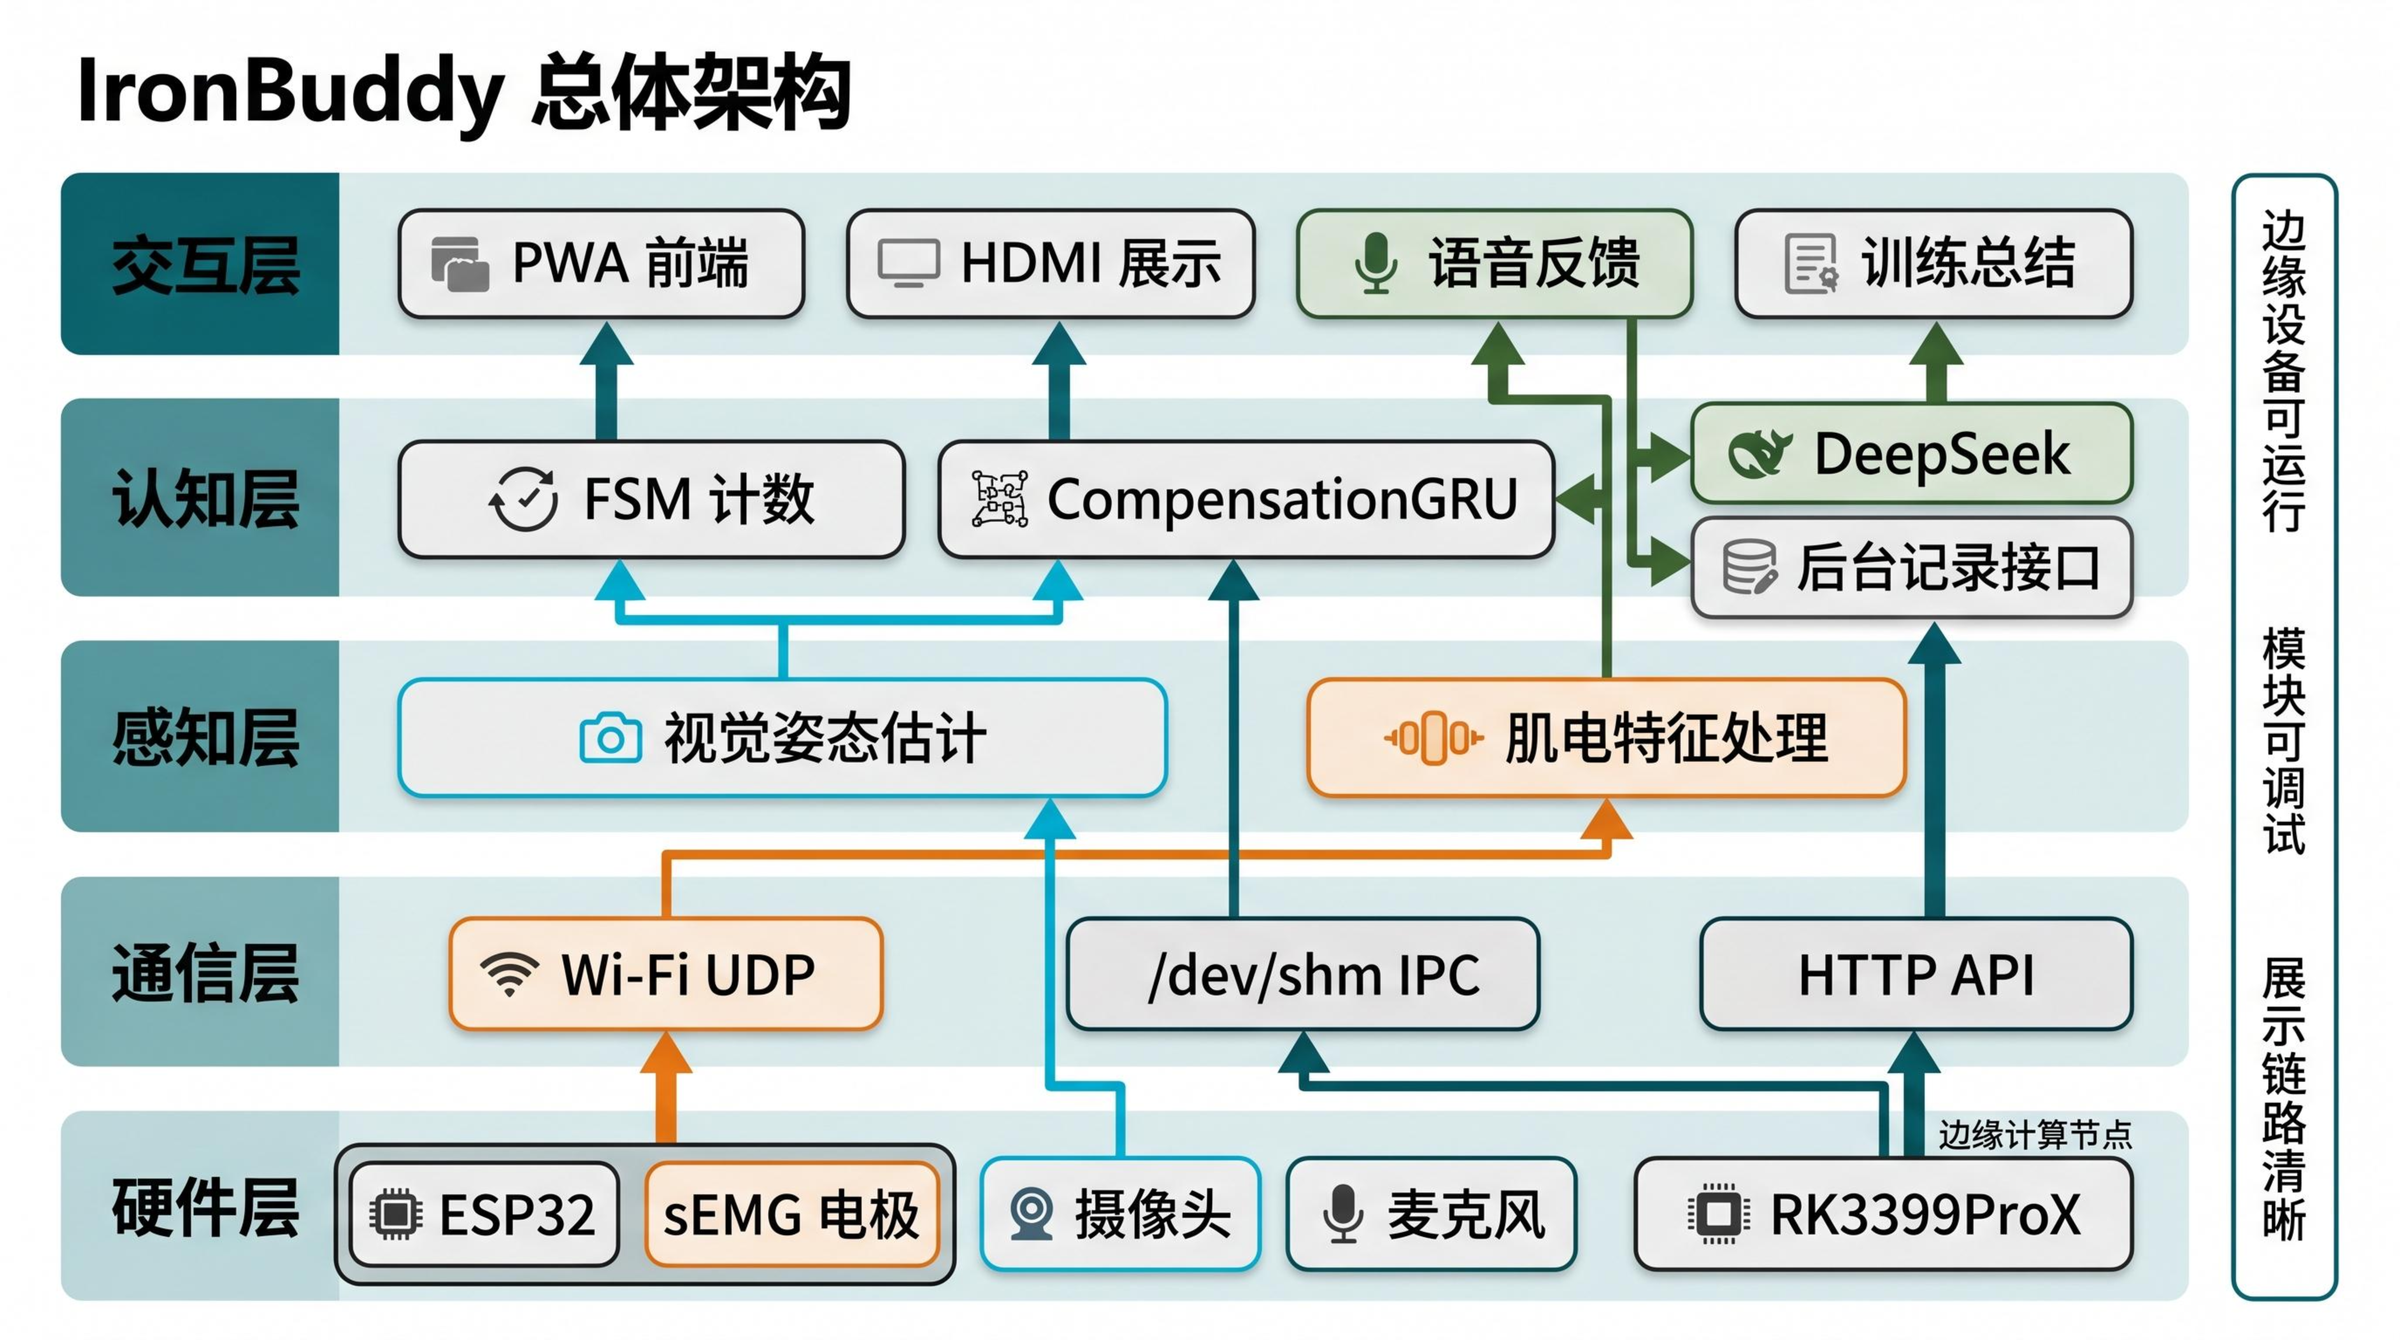
\includegraphics[width=0.92\textwidth]{figures/report/fig02.png}
    \caption{系统总体架构。}
    \label{fig:system-architecture}
\end{figure}

\subsection{软件总体：多进程与共享状态}

本节说明系统如何用多进程和共享状态把视觉、肌电、语音、前端与后台记录
隔离开。

\subsubsection{整体运行方式}

本项目的软件部分最终采用多进程结构。视觉、肌电、状态机、Web 服务和
语音逻辑分别运行，各自负责一类清楚的任务。早期把多种功能塞进同一主循环
时，摄像头、语音或前端任一环节卡住都会影响其他模块；拆分后，单个模块
异常更容易定位，也更适合现场调试。

\begin{table}[htbp]
\centering
\small
\begin{tabular}{@{}>{\raggedright\arraybackslash}p{0.23\textwidth}
                >{\raggedright\arraybackslash}p{0.31\textwidth}
                >{\raggedright\arraybackslash}p{0.34\textwidth}@{}}
\toprule
\textbf{模块} & \textbf{主要职责} & \textbf{典型输出} \\
\midrule
streamer\_app & Web 控制台、视频流、API 入口 & 页面状态、用户操作信号 \\
vision & 本地或云端姿态估计 & 关键点、关节角度、视觉模式 \\
main\_claw\_loop & FSM 计数、GRU 推理、训练状态 & 次数、动作质量、疲劳值 \\
udp\_emg\_server & 肌电 UDP 接收与特征处理 & 目标肌/代偿肌激活特征 \\
voice\_daemon & 语音唤醒、TTS、命令和对话 & 语音回复、动作切换、聊天状态 \\
\bottomrule
\end{tabular}
\caption{系统核心进程与职责划分}
\label{tab:processes}
\end{table}

这些进程之间主要通过 \code{/dev/shm} 下的 JSON 或文本文件交换状态。写入方
先写临时文件，再用 rename 替换正式文件，减少读到半截内容的概率。这个
方案不如消息队列完整，但它简单、透明、跨进程可见。调试时直接查看共享
状态文件，就能判断当前是视觉、肌电、FSM、语音还是前端出了问题。

\begin{figure}[htbp]
    \centering
    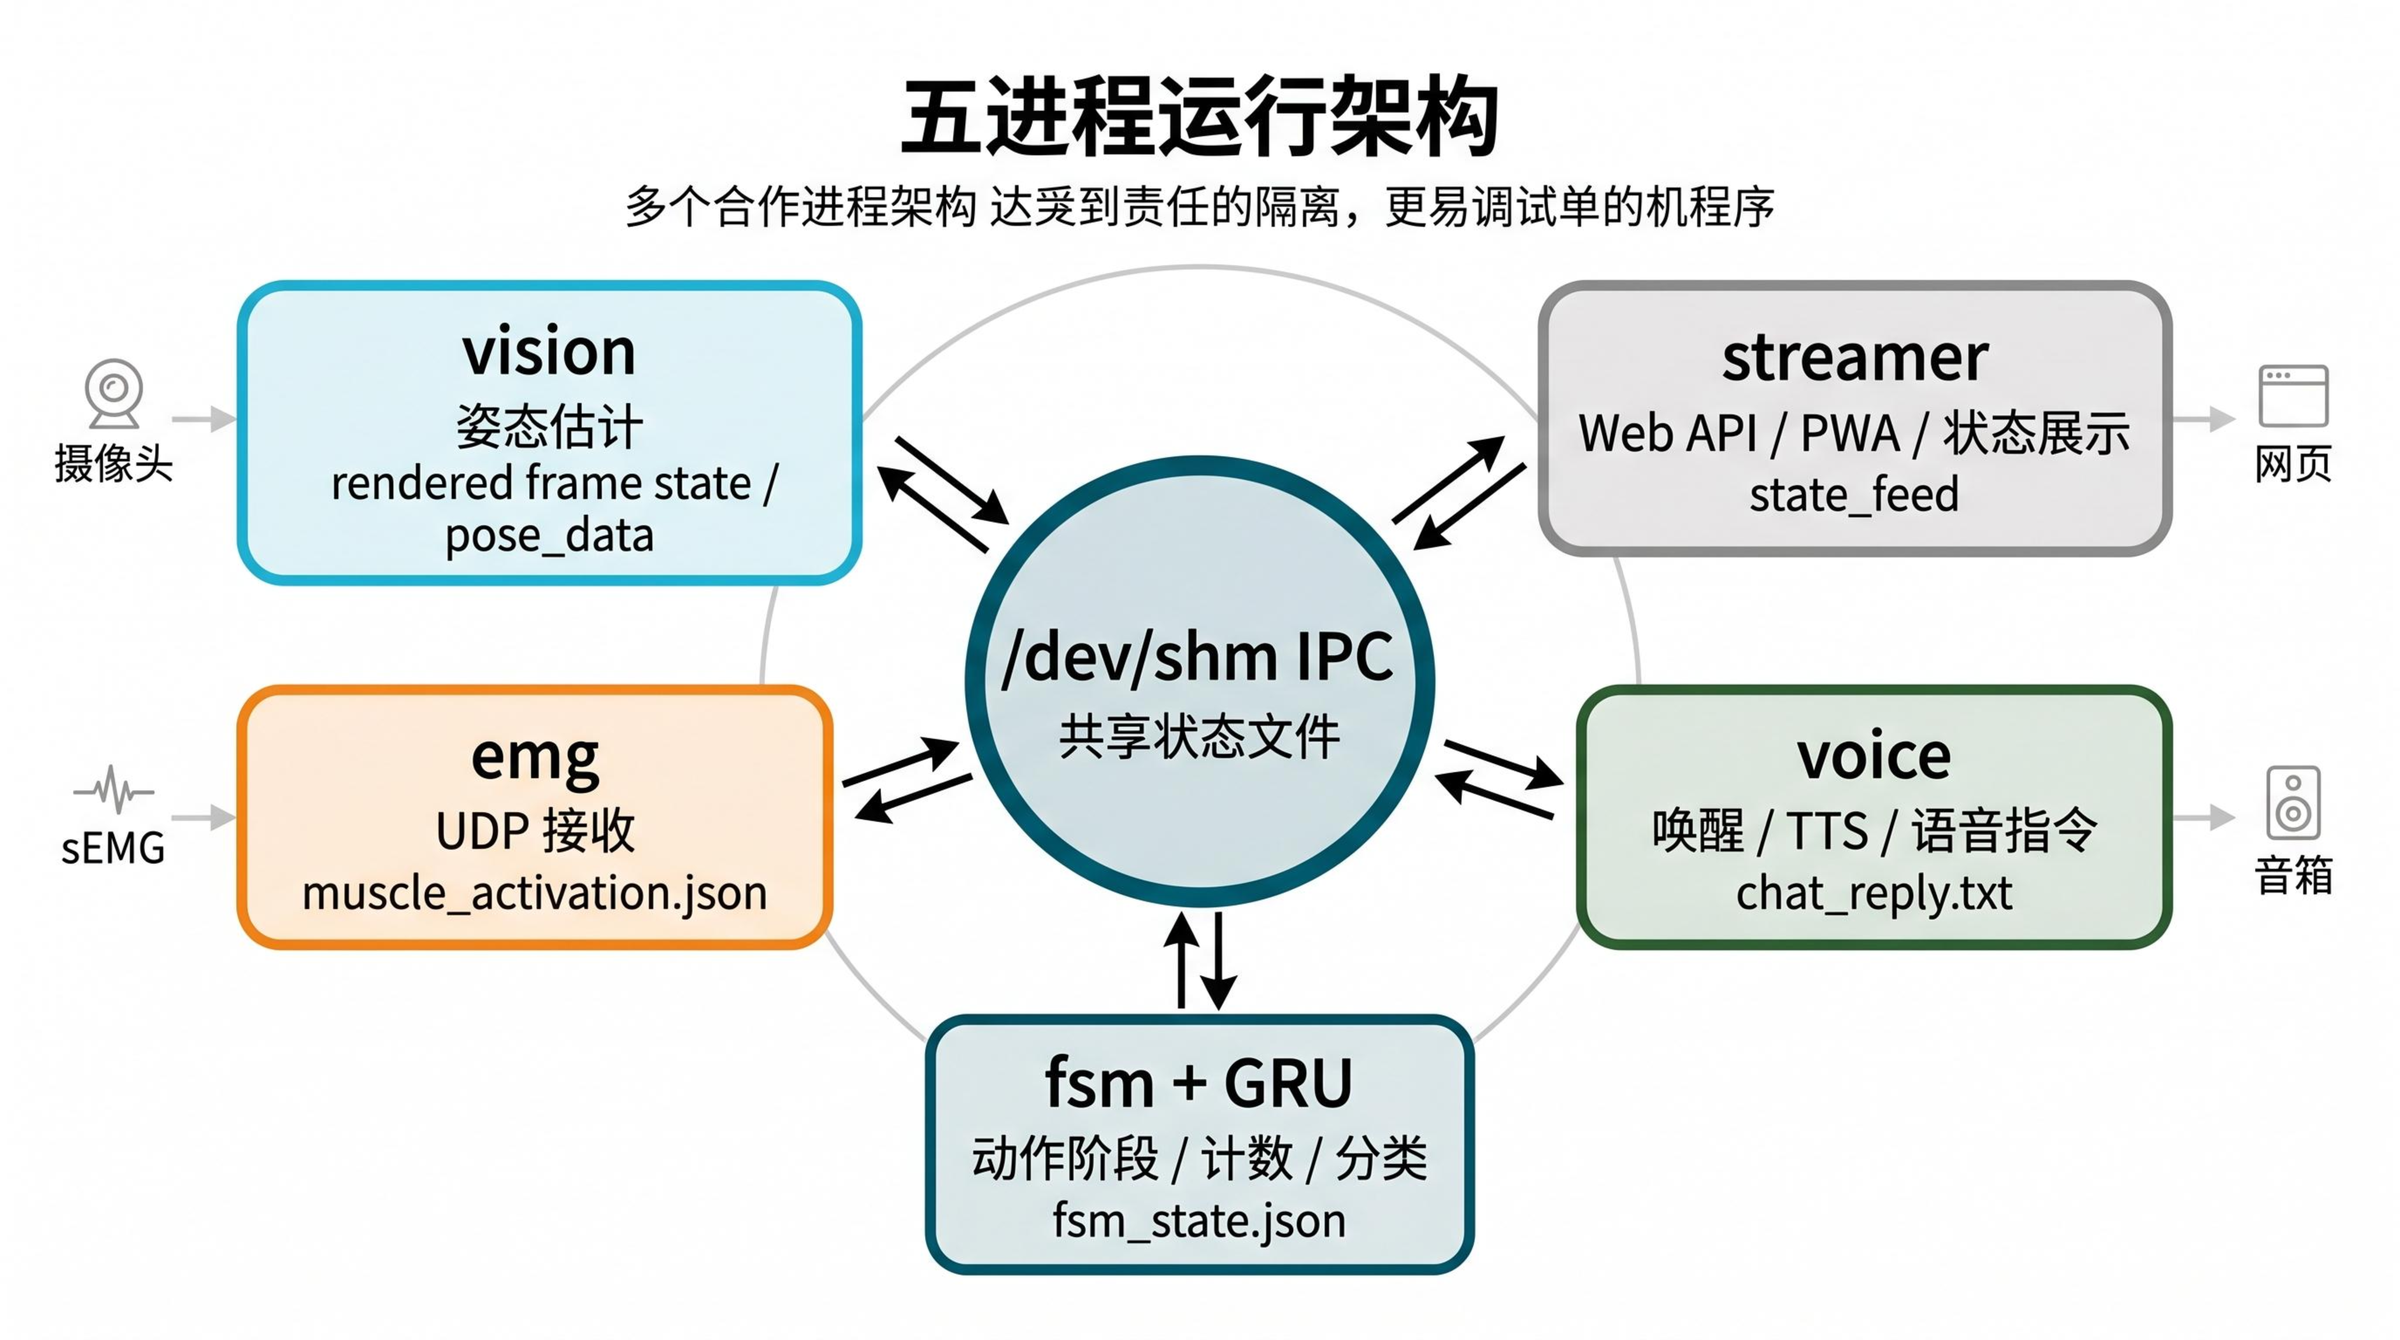
\includegraphics[width=0.9\textwidth]{figures/report/fig05.png}
    \caption{以共享状态文件为中心的进程协作方式。}
    \label{fig:ipc}
\end{figure}

\subsubsection{数据流与状态流}

一次训练中的数据流可以分为三条。第一条是视觉流：摄像头帧进入本地 NPU
或云端 RTMPose，输出关键点、关节角度和动作阶段参考。第二条是肌电流：
ESP32 将目标肌和代偿肌的采样特征通过 UDP 发送到板端，处理后写入肌肉
激活状态。第三条是交互流：用户通过语音或前端改变动作模式、疲劳上限和
视觉模式，系统再把这些意图写入共享状态文件。

这三条流最终在 FSM 和 GRU 处汇合。FSM 根据关节角度变化识别动作阶段和
完成次数，GRU 根据最近一段 7D 特征窗口判断动作质量，前端和语音再把这些
结果转化为可读反馈。这样的结构让每个模块都有明确输入和输出，也避免了
前端、语音和模型互相直接调用内部函数。

\begin{figure}[htbp]
    \centering
    \resizebox{0.96\textwidth}{!}{%
    \begin{tikzpicture}[
        node distance=0.65cm and 0.95cm,
        box/.style={draw, rounded corners=2pt, align=center, font=\small,
                    minimum height=0.72cm, minimum width=2.45cm},
        vision/.style={box, fill=cyan!9, draw=cyan!65!black},
        emg/.style={box, fill=orange!11, draw=orange!80!black},
        user/.style={box, fill=green!9, draw=green!55!black},
        state/.style={box, fill=teal!9, draw=teal!70!black, minimum width=3.0cm},
        judge/.style={box, fill=purple!7, draw=purple!55!black},
        outputbox/.style={box, fill=gray!8, draw=gray!65},
        arrow/.style={-{Latex[length=2mm]}, thick}
    ]
        \node[vision] (camera) {摄像头帧};
        \node[vision, right=of camera] (pose) {姿态估计\\关键点 / 角度};
        \node[emg, below=of camera] (esp) {ESP32 肌电};
        \node[emg, right=of esp] (emgfeat) {肌电特征\\RMS / MVC};
        \node[user, below=of esp] (intent) {用户意图\\语音 / 前端};
        \node[user, right=of intent] (mode) {训练参数\\动作 / 阈值};

        \node[state, right=1.25cm of pose, yshift=-0.72cm] (shm)
            {\code{/dev/shm}\\共享状态层};
        \node[judge, right=1.15cm of shm, yshift=0.58cm] (fsm)
            {FSM\\阶段 / 计数};
        \node[judge, right=1.15cm of shm, yshift=-0.58cm] (gru)
            {GRU\\质量判断};
        \node[outputbox, right=1.1cm of fsm] (feedback)
            {反馈输出\\语音 / 页面};
        \node[outputbox, right=1.1cm of gru] (record)
            {记录沉淀\\数据库 / 总结};

        \draw[arrow, cyan!70!black] (camera) -- (pose);
        \draw[arrow, orange!85!black] (esp) -- (emgfeat);
        \draw[arrow, green!60!black] (intent) -- (mode);
        \draw[arrow, cyan!70!black] (pose) -- (shm);
        \draw[arrow, orange!85!black] (emgfeat) -- (shm);
        \draw[arrow, green!60!black] (mode) -- (shm);
        \draw[arrow, teal!70!black] (shm) -- (fsm);
        \draw[arrow, teal!70!black] (shm) -- (gru);
        \draw[arrow, purple!60!black] (fsm) -- (feedback);
        \draw[arrow, purple!60!black] (gru) -- (feedback);
        \draw[arrow, purple!60!black] (fsm) -- (record);
        \draw[arrow, purple!60!black] (gru) -- (record);
    \end{tikzpicture}}
    \caption{训练过程中的数据流与状态流。}
    \label{fig:data-state-flow}
\end{figure}

\subsection{训练业务：从计数到结果导向}

在前面骨架基础上，本节描述训练业务如何从单纯计数转向兼顾目标肌激活与
代偿判断，并以一次完整流程为例说明各模块的协同。

\subsubsection{结果导向的训练方式}

本项目的一个重点是把训练记录从"做了几次"推进到"每次动作是否真正
练到了"。传统次数统计只能说明动作完成了多少个，却不能说明目标肌激活
是否充分，也不能区分标准发力和代偿发力。系统因此把次数放在基础层，把
目标肌激活、代偿肌比例和疲劳积分放在质量层。

具体落地参数上，视觉特征以 30 Hz 写入共享状态层，肌电特征以 100 Hz 由
ESP32 通过 UDP 上行后由板端聚合为 30 Hz 同步帧；GRU 推理在每一组动作
完成时触发一次，输入为最近 W=64 帧（约 2.1 s）的 7D 特征窗口，输出
标准 / 代偿 / 不标准三类。前端展示时，用户不仅看到完成次数，也能看到
疲劳积分、动作质量和代偿提示。疲劳积分是工程化训练负荷指标，综合完成
次数、动作质量与肌电激活趋势，用于提示本组训练是否接近上限；表面肌电
频域指标也常用于评估肌肉疲劳趋势 \cite{cifrek2009}，但本项目的疲劳
积分仅作为反馈和展示指标使用，不写为生理疲劳的严格度量。

\begin{algorithm}[htbp]
\caption{每帧 FSM 计数与 GRU 质量判断（以深蹲为例）}
\label{alg:fsm-gru}
\begin{algorithmic}[1]
\Require pose, emg from \texttt{/dev/shm}; thresholds $\theta_{\text{down}}, \theta_{\text{up}}$; window $W$
\State $f_t \gets$ Build7DFeature(pose, emg)
\Statex \quad \Comment{角度 / 角速度 / 角加速度 / 目标肌 RMS / 代偿肌 RMS / 对称性 / 相位}
\State Push $f_t$ into ring buffer of length $W$
\If{state $=$ UP $\land$ knee\_angle $< \theta_{\text{down}}$}
    \State state $\gets$ DOWN
\ElsIf{state $=$ DOWN $\land$ knee\_angle $> \theta_{\text{up}}$}
    \State state $\gets$ UP; \quad count $\mathrel{+}{=} 1$
    \State $y \gets$ \Call{GRU}{$f_{t-W+1:t}$}
    \Statex \quad \Comment{$y \in \{\text{good}, \text{compensated}, \text{bad}\}$}
    \State Append (count, $y$, fatigue) to \texttt{/dev/shm/rep\_event.json}
    \If{$y \neq \text{good}$} \State TriggerVoiceFeedback($y$) \EndIf
\EndIf
\end{algorithmic}
\end{algorithm}

算法 \ref{alg:fsm-gru} 也解释了为什么系统没有完全依赖神经网络计数：
计数本身是几何问题，用 FSM 更稳定；代偿识别才需要模型综合多个信号。
两者分工后，系统既能保留规则的可解释性，又能利用肌电补充纯视觉看不到
的信息。

\subsubsection{一次典型训练流程}

从用户视角看，一次训练可以自然串起上述模块。用户穿戴腰包、贴片和传感
线路后，通过语音或前端选择动作模式；视觉模块识别身体姿态，肌电模块上传
目标肌和代偿肌特征；FSM 根据动作阶段计数，GRU 在动作窗口内判断质量；
前端显示训练状态，语音在动作切换、MVC、疲劳接近上限或用户主动询问时
给出反馈。

这个流程的关键不是某个模块单独"很强"，而是各模块之间不要互相抢控制权。
前端可以写入疲劳上限，语音也可以写入；FSM 会触发总结，用户也可能正在
对话；TTS 播报时麦克风仍能听到声音。项目用共享状态文件、时间戳和状态机
把这些行为隔离开，使系统在功能越来越多时仍然保持可读和可调试。

\begin{figure}[htbp]
    \centering
    \resizebox{0.96\textwidth}{!}{%
    \begin{tikzpicture}[
        lane/.style={font=\bfseries\small, anchor=east},
        evt/.style={draw, rounded corners=2pt, fill=cyan!10, draw=cyan!65!black,
                    font=\scriptsize, inner sep=2.5pt, minimum height=0.55cm},
        evt2/.style={evt, fill=orange!12, draw=orange!75!black},
        evt3/.style={evt, fill=purple!9, draw=purple!60!black},
        evt4/.style={evt, fill=green!11, draw=green!55!black},
        evt5/.style={evt, fill=teal!11, draw=teal!70!black},
        ax/.style={->, gray!60, thick}
    ]
    % 五条泳道
    \foreach \y/\name in {0/用户, -1/视觉, -2/肌电, -3/FSM/GRU, -4/反馈}
        \node[lane] at (-0.2,\y) {\name};
    % 时间轴
    \foreach \y in {0,-1,-2,-3,-4}
        \draw[ax] (0,\y) -- (15.5,\y);
    \node[font=\scriptsize, anchor=west] at (15.5,-2) {$t$};

    % 事件块 (时间, lane, 类型, 文字)
    \node[evt5] at (1.2,0) {唤醒"教练"};
    \node[evt5] at (3.2,0) {选择动作};
    \node[evt4] at (5.7,0) {开始第 1 组};
    \node[evt4] at (12.6,0) {主动询问};

    \node[evt] at (5.7,-1) {骨架@30Hz};
    \node[evt] at (8.5,-1) {阶段=DOWN};
    \node[evt] at (10.2,-1) {阶段=UP};
    \node[evt] at (13.5,-1) {骨架@30Hz};

    \node[evt2] at (5.7,-2) {RMS@100Hz};
    \node[evt2] at (8.5,-2) {激活峰值};
    \node[evt2] at (10.2,-2) {代偿信号};
    \node[evt2] at (13.5,-2) {RMS@100Hz};

    \node[evt3] at (8.5,-3) {计数+1};
    \node[evt3] at (10.4,-3) {GRU=代偿};
    \node[evt3] at (12.0,-3) {疲劳累积};

    \node[evt5] at (3.2,-4) {TTS 引导};
    \node[evt5] at (10.6,-4) {语音提示};
    \node[evt5] at (12.8,-4) {DeepSeek 答复};

    % 关键依赖箭头
    \draw[->, dashed, gray!70] (8.5,-1) -- (8.5,-2.7);
    \draw[->, dashed, gray!70] (8.5,-2) -- (8.5,-2.85);
    \draw[->, dashed, gray!70] (10.2,-1) -- (10.4,-2.7);
    \draw[->, dashed, gray!70] (10.2,-2) -- (10.4,-2.85);
    \draw[->, dashed, gray!70] (10.4,-3) -- (10.6,-3.7);
    \draw[->, dashed, gray!70] (12.6,0) -- (12.8,-3.7);
    \end{tikzpicture}}
    \caption{一次完整训练的多模块时序示意。}
    \label{fig:training-timeline}
\end{figure}

\subsection{交互与维护：语音、调试控制台与数据库}

交互层与维护层共享同一套状态文件。本节说明语音状态机、调试控制台和
数据库如何让系统在功能扩展时仍可复测。

\subsubsection{语音交互与冲突仲裁}

语音模块面向的是运动中的真实操作场景。用户可能正在拿哑铃、做深蹲或佩戴
贴片，此时触屏并不自然。系统因此把动作切换、疲劳上限调整、MVC 引导、
训练总结和简单问答都接入语音链路，让前端更多承担展示和调试入口。

语音链路的难点在于冲突仲裁。用户主动唤醒、系统自动总结和 TTS 播报可能
同时发生；如果没有状态管理，系统播报的声音还可能被麦克风录回去。后期
重构把语音逻辑整理为 LISTEN、DIALOG、BUSY 三个状态。LISTEN 等待唤醒，
DIALOG 处理用户一轮指令或问答，BUSY 处理 TTS、MVC 流程和自动总结。BUSY
期间暂停录音，降低自录和串音风险。

\begin{figure}[htbp]
    \centering
    \resizebox{0.82\textwidth}{!}{%
    \begin{tikzpicture}[
        state/.style={draw, rounded corners=3pt, align=center, minimum width=3.0cm,
                      minimum height=1.0cm, font=\small},
        listen/.style={state, fill=teal!12, draw=teal!70!black},
        dialog/.style={state, fill=green!10, draw=green!55!black},
        busy/.style={state, fill=orange!14, draw=orange!80!black},
        note/.style={draw, rounded corners=2pt, align=center, fill=red!5,
                     draw=red!45!black, font=\small, minimum width=3.8cm},
        arrow/.style={-{Latex[length=2mm]}, thick}
    ]
        \node[listen] (listen) {LISTEN\\等待唤醒 / 监听"教练"};
        \node[dialog, right=3.4cm of listen] (dialog) {DIALOG\\识别指令 / 调用对话或工具};
        \node[busy, below=2.1cm of dialog] (busy) {BUSY\\TTS 播报 / MVC 流程 / 自动总结};
        \node[note, left=2.1cm of busy] (note) {BUSY 期间暂停录音\\减少 TTS 被再次录入};

        \draw[arrow, teal!70!black] (listen) -- node[above, font=\small]{唤醒词或语音指令} (dialog);
        \draw[arrow, green!55!black] (dialog) -- node[right, font=\small]{生成回复或触发流程} (busy);
        \draw[arrow, orange!80!black] (busy.west) -- ++(-1.0,0) |- node[pos=0.24, left, font=\small]{播报完成 / 流程结束} (listen.south);
        \draw[arrow, gray!70!black] (dialog.north) to[bend left=30]
            node[above, font=\small]{没听清或超时归位} (listen.north);
        \draw[arrow, red!55!black] (note) -- (busy);
    \end{tikzpicture}}
    \caption{语音模块的三状态模型。}
    \label{fig:voice-state}
\end{figure}

\subsubsection{统一状态观察与端到端调试控制台}

系统进入后期后，主要困难不再是单个功能能否跑通，而是如何在一个已经成型
的端到端项目中继续升级。视觉、肌电、FSM、语音、LLM、数据库和 Web 前端
之间存在大量状态依赖；如果只凭直觉修改代码，很容易修好一个局部，又在
另一条链路上引入新问题。因此，本项目搭建了一套面向多模块协同维护的
端到端调试控制台，把状态观察、问题定位、修改建议和复测记录组织成固定流程。

这套工作台的核心不是增加一个独立页面，而是建立可被人和工具共同读取的
调试表征。系统把关键运行状态、知识库命中、云端记忆、数据库记录、代码
结构关系和测试步骤整理到统一入口中。这样在添加新功能或修复旧问题时，
可以先确认当前现象，再定位涉及的模块和状态文件，随后根据复测记录检查
修改是否真的改善了端到端结果。

这种设计让外部协作者不必从零理解项目，也能围绕真实运行状态、历史记录和
代码结构提出修改建议，再根据复测结果决定是否保留。对于包含多进程、
传感器、语音和前端的系统来说，这种结果导向的调试方式比盲目重构更稳，
也更适合后续长期维护。

\begin{figure}[htbp]
    \centering
    \resizebox{0.92\textwidth}{!}{%
    \begin{tikzpicture}[
        center/.style={draw, rounded corners=4pt, align=center,
                       fill=teal!13, draw=teal!70!black, font=\bfseries\small,
                       minimum width=3.4cm, minimum height=1.1cm},
        panel/.style={draw, rounded corners=3pt, align=center, font=\small,
                      minimum width=3.0cm, minimum height=0.95cm},
        p1/.style={panel, fill=cyan!10, draw=cyan!65!black},
        p2/.style={panel, fill=orange!11, draw=orange!75!black},
        p3/.style={panel, fill=purple!8, draw=purple!60!black},
        p4/.style={panel, fill=green!10, draw=green!55!black},
        p5/.style={panel, fill=red!7, draw=red!55!black},
        arrow/.style={-{Latex[length=2mm]}, thick, gray!70}
    ]
        \node[center] (hub) at (0,0) {端到端调试控制台\\\scriptsize ironbuddy\_operator\_console};
        \node[p1] (a) at (-5.5, 1.6) {运行状态\\\scriptsize 5 个进程心跳};
        \node[p2] (b) at (-5.5,-1.6) {传感验证\\\scriptsize 视频 / EMG 波形};
        \node[p3] (c) at ( 0, 2.6) {知识库命中\\\scriptsize RAG-lite 检索};
        \node[p4] (d) at ( 5.5, 1.6) {数据库视图\\\scriptsize 5 张表 + 记录};
        \node[p5] (e) at ( 5.5,-1.6) {代码结构关系\\\scriptsize 模块依赖图};
        \node[panel, fill=gray!8, draw=gray!60] (f) at ( 0,-2.6) {复测记录\\\scriptsize 手测脚本 + 截图};

        \draw[arrow] (a) -- (hub); \draw[arrow] (b) -- (hub);
        \draw[arrow] (c) -- (hub); \draw[arrow] (d) -- (hub);
        \draw[arrow] (e) -- (hub); \draw[arrow] (f) -- (hub);
    \end{tikzpicture}}
    \caption{端到端调试控制台的六个观察面板。}
    \label{fig:debug-console}
\end{figure}

\subsubsection{训练记录与长期接口}

训练系统如果只看当前一组动作，很难在后续迭代中复盘问题。本项目因此
保留了本地数据库和训练记录接口：每次训练产生的动作、疲劳、对话和总结
都可以沉淀为后续分析材料。数据库不仅保存记录，也为后续模型迭代、训练
周报、偏好学习和个性化建议留下接口。

\begin{figure}[htbp]
    \centering
    \begin{subfigure}[t]{0.46\textwidth}
        \centering
        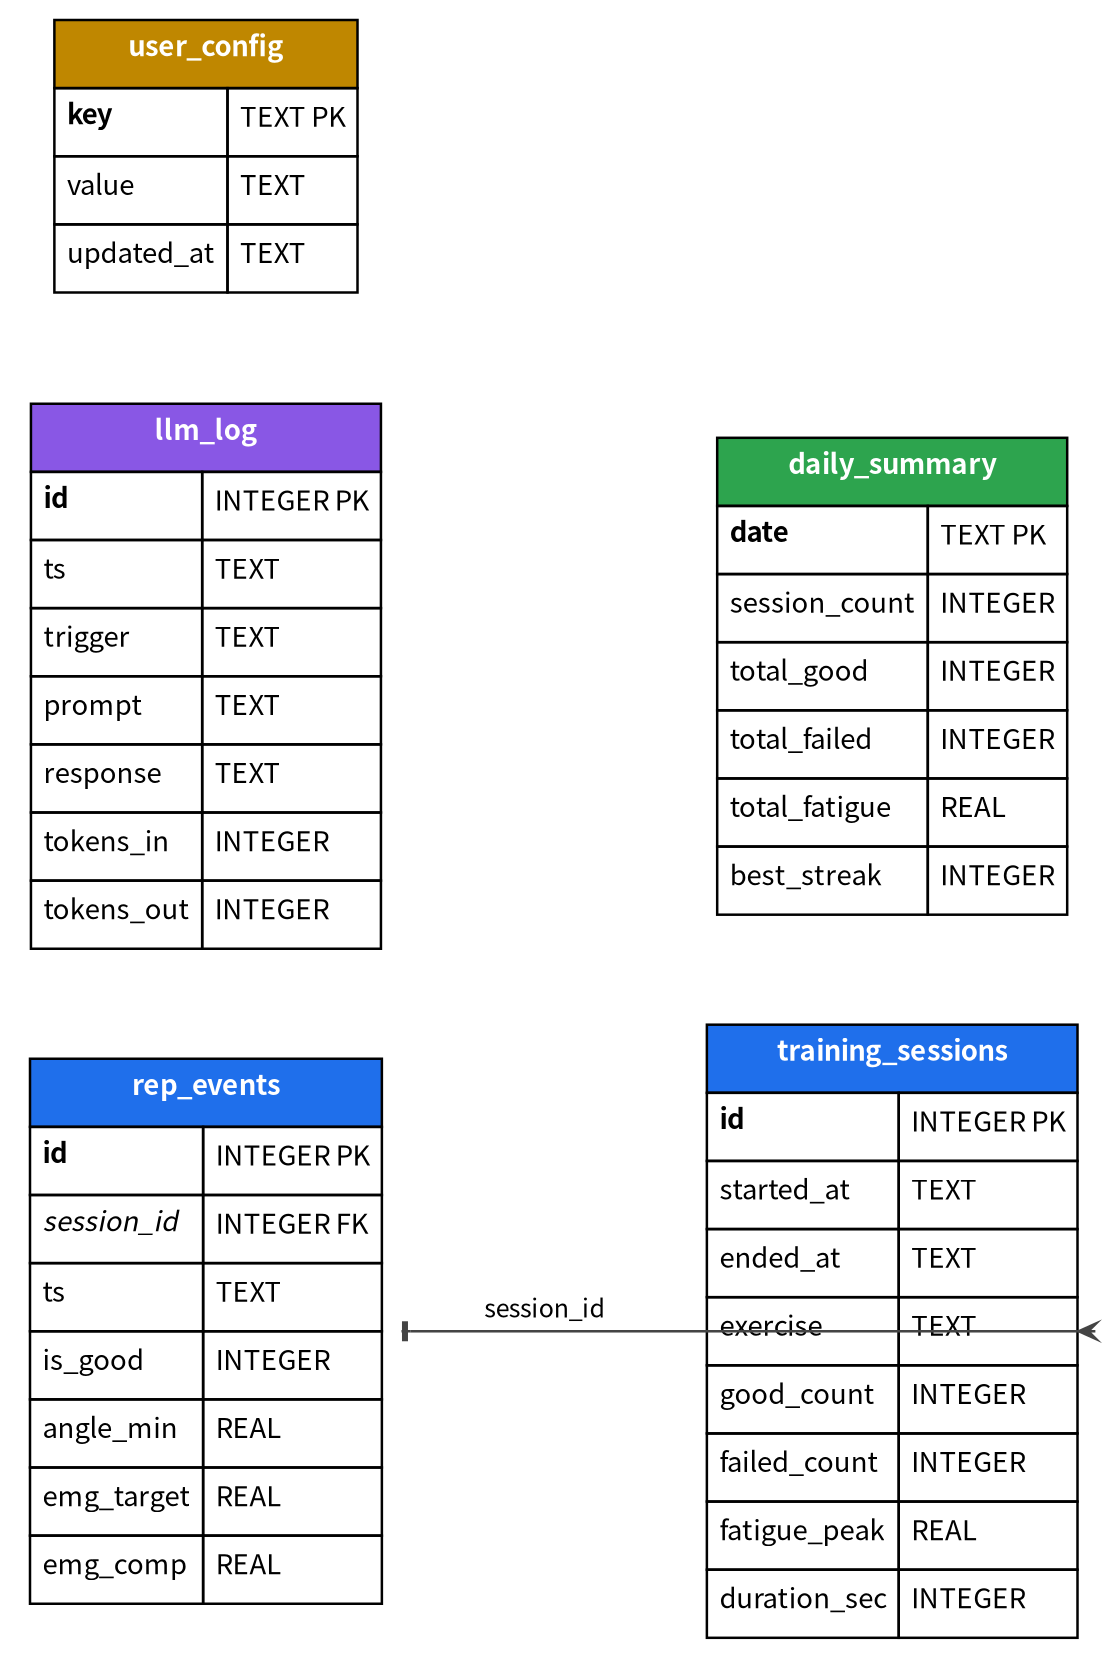
\includegraphics[width=\linewidth]{figures/report/fig09a-er.png}
        \caption{表关系（ER）视图}\label{fig:db-er}
    \end{subfigure}\hfill
    \begin{subfigure}[t]{0.50\textwidth}
        \centering
        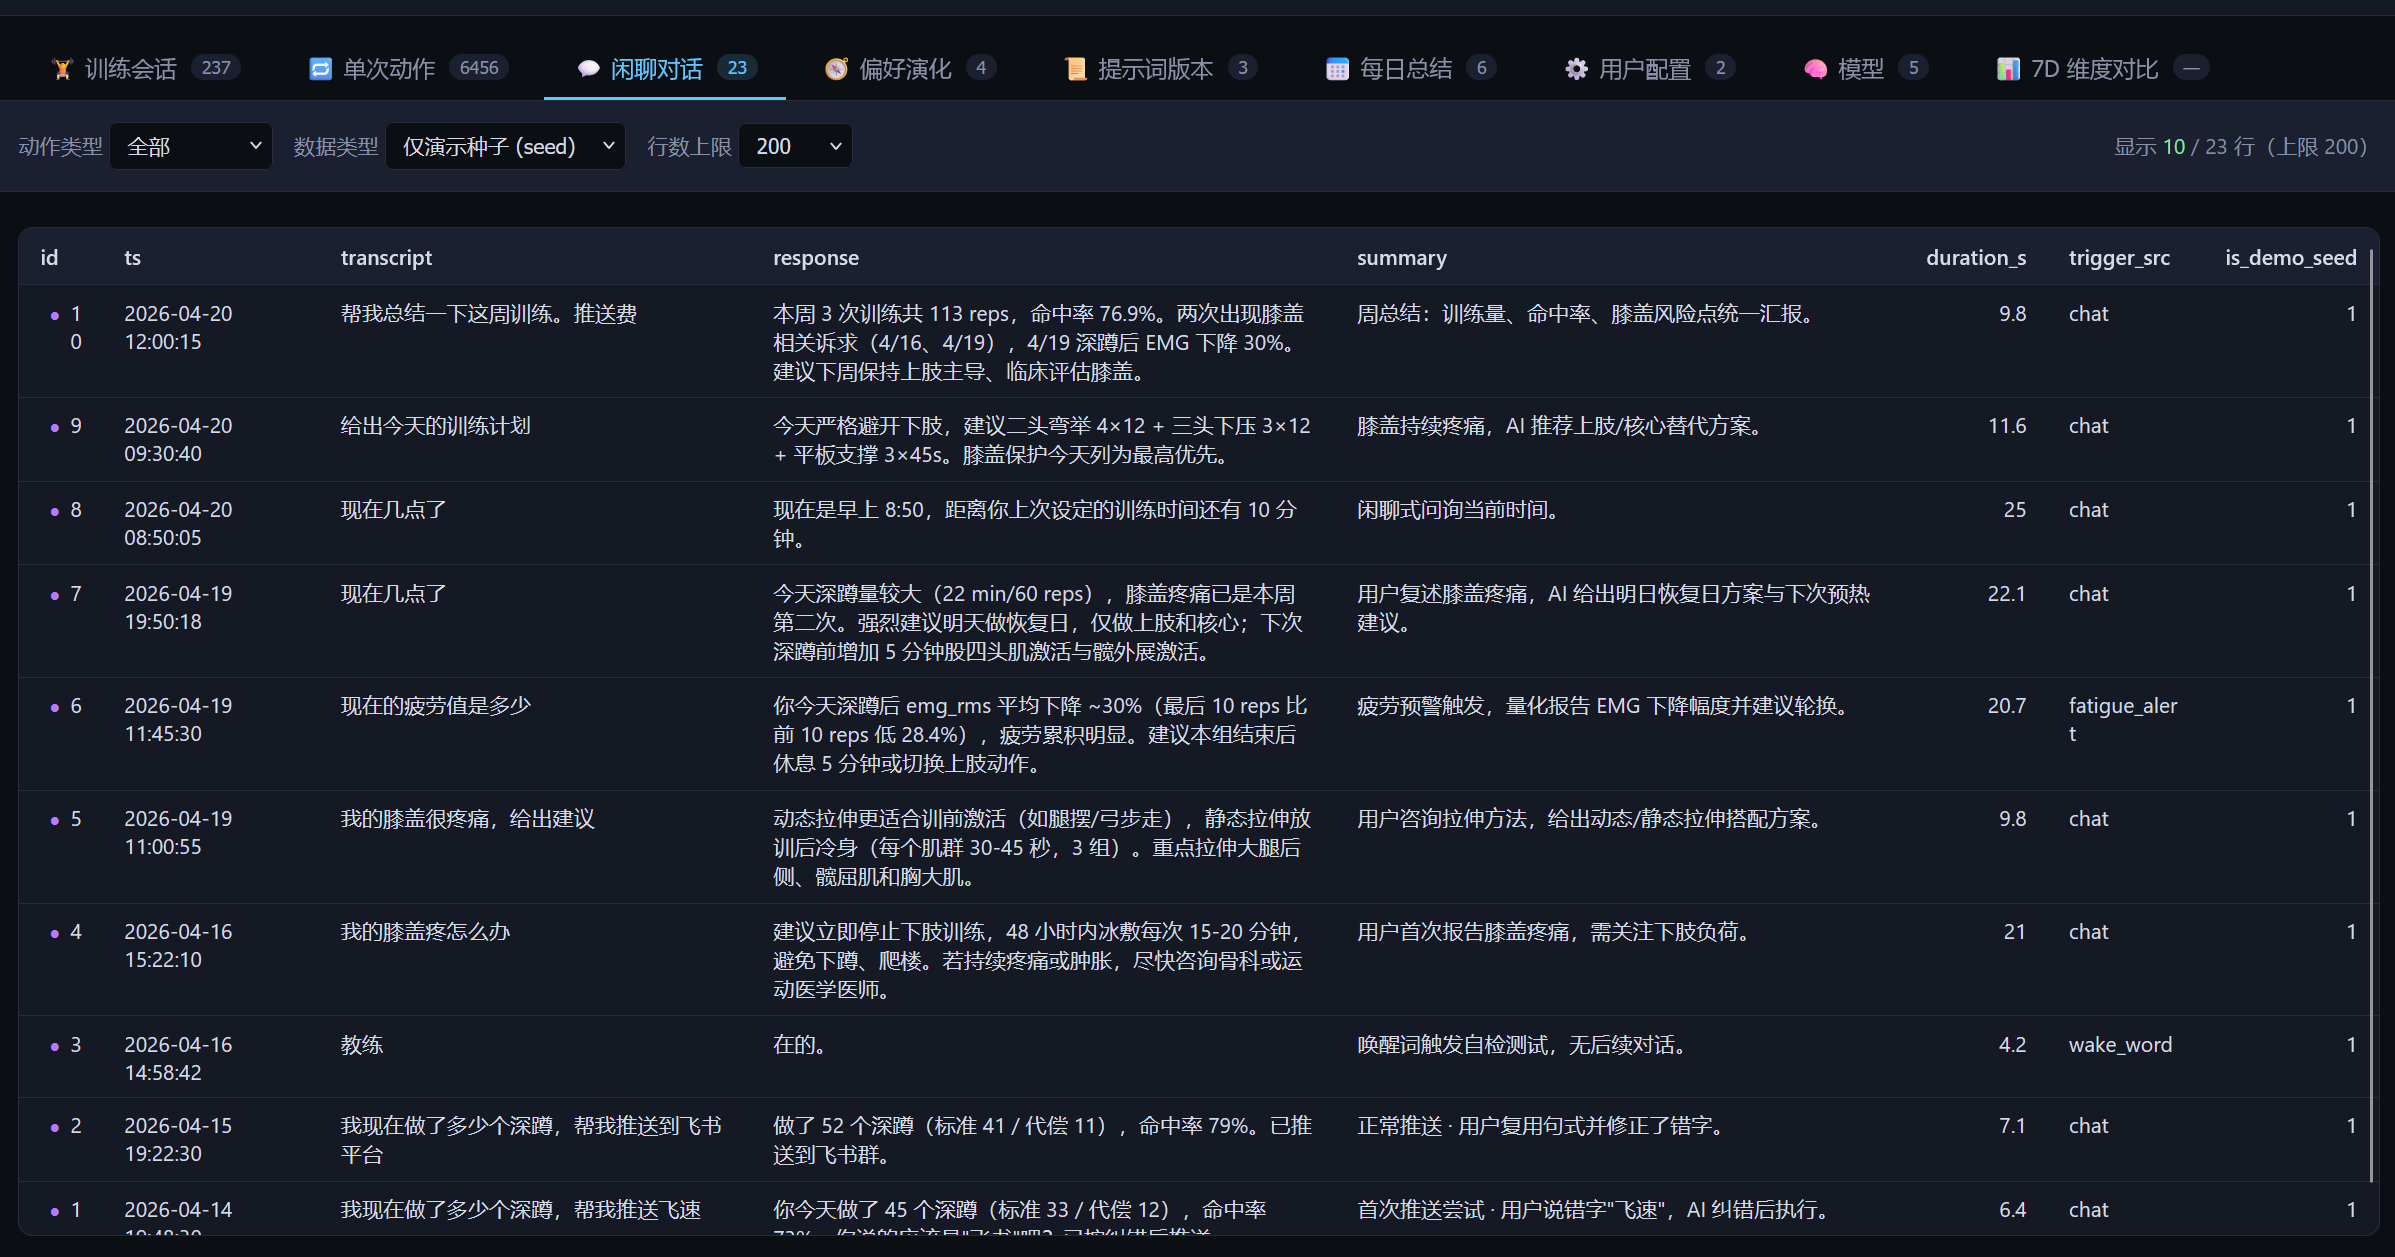
\includegraphics[width=\linewidth]{figures/report/fig09b-record.png}
        \caption{对话记录子表示例}\label{fig:db-record}
    \end{subfigure}
    \caption{本地训练记录数据库的 ER 视图与记录示例（5 张表：\texttt{training\_sessions} 训练会话、\texttt{rep\_events} 单次动作、\texttt{llm\_log} 对话日志、\texttt{daily\_summary} 每日总结、\texttt{user\_config} 用户配置）。}
    \label{fig:database}
\end{figure}

数据库记录为长期个性化分析预留了数据基础，能够把训练过程、用户问题、
总结文本和偏好变化沉淀下来。随着真实训练数据和复测流程继续积累，这些
记录可以进一步支持用户偏好建模、周期性训练总结和更稳定的个性化建议。

\subsection*{本章小结}
\addcontentsline{toc}{subsection}{本章小结}

本章把 IronBuddy 的软件层拆成总体架构、训练业务和交互维护三层。多进程
与共享状态保证了模块边界，结果导向的训练业务把计数推进到了质量判断，
语音状态机、调试控制台和本地数据库则让系统在功能持续扩展时仍能保持
可读、可复测。

\section{工程调试与问题复盘}
\label{sec:debug}

本项目的开发过程里，最有价值的部分不只是功能逐步增加，也包括一些
真正改变设计的调试经历。本章保留几个对系统形态影响较大的问题，重点说明
它们如何影响后续取舍。

\subsection{语音链路的底层排查}

语音是项目中最早让系统“像教练”的模块，也是最容易误判根因的模块。起初
使用摄像头自带的数字音频输入，延迟和识别率都不理想；后来换到板端麦克风
链路后，又遇到唤醒词不稳定、录音为空、ALSA 设备被占用等问题。

这些问题一开始很容易被归因到语音识别代码。但单独跑录音测试后可以发现，
真正麻烦的是音频设备句柄、采样率初始化、旧守护进程残留和 TTS/录音抢
设备等问题交织在一起。于是项目后期把语音调试拆成更小的链路：先确认录音
文件，再确认 ASR 返回，再进入唤醒词、命令路由和 TTS 播报。

这次经历带来的教训是，嵌入式项目里不能只在最终业务模块里查问题。音频、
摄像头、网络和传感器都需要先有最小可复现测试。只有确认底层采集链路是
干净的，再回到业务逻辑里看状态机和路由，才不会反复怀疑错误对象。

\subsection{肌电输入的佩戴影响}

肌电问题也有类似特点。早期波形不稳定时，直觉上会怀疑电源、放大电路或
代码解析。但实际测试中，贴片是否贴紧、皮肤是否潮湿、线缆是否晃动，都会
影响采样结果。贴片接触不好时，模型端再怎么调整也很难得到稳定判断。

这也是项目后来强调规范穿戴流程和 MVC 归一化的原因。模型再轻量、代码再
整洁，如果输入本身漂移很大，最终判断仍然会不稳定。与其在模型端不断补
规则，不如先把佩戴、采样和归一化流程固定下来。

\subsection{功能叠加后的重新分层}

项目后期另一个明显问题是代码耦合。每加一个功能，最简单的做法都是在旧的
主循环或前端逻辑里再加一段 if/else。但这种做法积累到一定程度后，调试
成本会快速上升：一个语音命令可能同时影响前端、FSM、LLM、TTS 和状态文件，
任何一处插入不当都会引发连锁问题。

V7.30 前后的整理没有推翻整个系统，而是把几个高频冲突点拆开：语音状态、
turn 协议、DeepSeek client、tools/router、auto trigger 和后台记录接口。
整理后代码不一定立刻变少，但入口更清楚，后续手测、拍摄和复盘也更容易
定位问题。

\subsection{调试工作台的价值}

随着模块增多，单靠终端日志很难支撑排查。第 \ref{sec:implementation} 章
描述的端到端调试控制台在工程意义上的价值，是把"系统当前处于哪一个
状态"从一个需要查日志和源码才能回答的问题，变成一个查面板就能回答
的问题。

这种工作台思路也改变了报告和演示的组织方式。过去更容易只讲“功能能做
什么”，现在可以讲清楚“系统如何被维护”。对于一个包含视觉、肌电、语音、
LLM 和 Web 的嵌入式项目来说，可维护性本身就是完成度的一部分。


\section{项目总结与展望}
\label{sec:conclusion}

\subsection{项目完成情况}

IronBuddy 最终形成的是一套模块边界清晰、可调试可复测的嵌入式健身教练系统。它把视觉
姿态估计、肌电传感、FSM 计数、GRU 动作质量判断、语音交互、Web 展示和
后台记录接口放在同一套系统里，围绕“动作是否标准、目标肌是否真正参与、
用户如何自然交互”建立了一条较完整的原型主线。

项目的主要收获不只是某个模型或某块硬件，而是多个模块之间的工程整合。
视觉模块解决外部姿态，肌电模块补充内部发力，状态机和 GRU 分别处理
确定性计数与模糊质量判断，语音和 LLM 让系统能以更自然的方式给用户反馈，
端到端调试系统和数据库则让系统维护与长期记录有了入口。

\subsection{仍然存在的不足}

项目也有明显不足。首先，肌电数据规模仍然有限，尤其是跨用户泛化能力不能
只根据本地训练表现下结论。贴片位置、皮肤状态和不同人的肌肉基础值都会
影响输入分布，真实 ESP32 UDP 连续输入也需要继续排查和复测。

其次，语音链路虽然已经做了状态化整理，但最终效果仍依赖现场麦克风距离、
网络状态、ASR 质量和 TTS 播报时机。工具调用、自动疲劳触发和 turn 去重
已经有代码与离线测试支撑，但仍需要完整手测后才能写成稳定结论。

再次，当前硬件形态更偏原型验证。腰包、外接线和贴片方便调试，却不是最终
产品形态。如果继续往产品化方向走，需要考虑贴片固定、小型化电源、外壳
结构、续航、无线稳定性和安全走线。

\subsection{后续方向}

后续可以从三个方向继续推进。

\begin{enumerate}
    \item \term{硬件集成与穿戴优化}：把采集板、ESP32 主控和电源集成到
    一块自制集成板中，通过更短线路提升装配便利性和佩戴安全性。运动服、
    腰包和肩带也可以进一步配合走线，让设备更适合真实训练动作。

    \item \term{扩展动作库和数据集}：在深蹲和弯举之外，继续覆盖硬拉、
    推举、划船等动作。每扩展一个动作，都需要重新确认目标肌和代偿肌、
    贴片位置、动作阶段和训练数据。

    \item \term{完善测试和长期记录}：把手测表、训练脚本、端到端调试系统、
    数据库记录和后台总结结合起来，形成固定的复测流程。
    这样每次改语音、模型或前端，都能判断是否影响主线演示。
\end{enumerate}

\subsection{个人体会}

IronBuddy 是我第一次完整经历从前端到后端、从软件到硬件的端到端项目。
之前的课程作业大多围绕单点问题展开：写一段算法、调一块电路、做一个
Demo 页面就算完成；而这次我必须同时面对完全不同性质的工程对象——
模拟前端的肌电采样和噪声、ESP32 的固件与无线链路、RK3399ProX 板端的
多进程与共享内存、本地 NPU 的 RKNN 量化模型、云端 GPU 的 RTMPose 推理
服务、Flask Web 服务和 PWA 前端、百度 AipSpeech 语音守护进程、DeepSeek
LLM 直连，以及 SQLite 长期记录。任何一个环节都不只是"能不能跑通"
的问题，更涉及"它在出错时长什么样、能不能被定位、改动之后会不会
破坏其他链路"。

真正实践之后才发现，跑通一个嵌入式全栈项目需要进行的 debug 数量是
超出想象的：贴片在运动中会移位、ALSA 在板端掉电后默认静音、子进程
必须用 bracket-trick 才能干净地 pgrep 出来、UDP 偶尔丢包却比 BLE
重传更适合连续传感、状态文件必须 write-then-rename 才能避免读到
半截 JSON、RKNN 量化模型的置信度阈值要从 0.5 降到 0.1 才适配板端
NPU、语音播报和麦克风录入需要状态机隔离才不会自录成回声。这些坑
没有一条来自单门课程，但合起来构成了嵌入式全栈系统能否真正稳定运行
的关键。

把这些散落在硬件、固件、操作系统、网络、AI 推理、Web 与语音之间的
碎片串成一条可运行、可调试的链路，是这门课程给我最大的工程收获。它
让我对"嵌入式系统"这四个字的理解从"在板子上跑一段代码"扩展到了
"让传感、算力、前端和用户在同一条反馈回路里协同工作"。也是从这门
课开始，我真正具备了去独立承担一个端到端嵌入式 AI 项目的工程能力，
能够在复杂依赖关系下做出取舍、定位问题、并把系统逐步推向稳定可用。

回过头看，IronBuddy 还不是一个可直接产品化的成品，但它已经回答了
最初提出的问题：当视觉与肌电互相补位时，居家健身系统可以从看动作
姿态走向理解动作背后的发力质量；而这条路要走通，需要的远不止一个
模型，更是一整套硬件、嵌入式软件、AI 推理与人机交互协同设计的能力。

\clearpage

\section*{参考文献}
\addcontentsline{toc}{section}{参考文献}

\begin{thebibliography}{9}
\bibitem{seniam}
Hermens, H. J., Freriks, B., Disselhorst-Klug, C., and Rau, G.
\newblock Development of recommendations for SEMG sensors and sensor placement
procedures.
\newblock \emph{Journal of Electromyography and Kinesiology}, 10(5):361--374,
2000.

\bibitem{burden2010}
Burden, A.
\newblock How should we normalize electromyograms obtained from healthy
participants? What we have learned from over 25 years of research.
\newblock \emph{Journal of Electromyography and Kinesiology}, 20(6):1023--1035,
2010.

\bibitem{cede2020}
Besomi, M., Hodges, P. W., Van Dieen, J., et al.
\newblock Consensus for experimental design in electromyography: Amplitude
normalization matrix.
\newblock \emph{Journal of Electromyography and Kinesiology}, 53:102438, 2020.

\bibitem{rtmpose}
Jiang, T., Lu, P., Zhang, L., et al.
\newblock RTMPose: Real-Time Multi-Person Pose Estimation based on MMPose.
\newblock arXiv:2303.07399, 2023.

\bibitem{mmpose}
Contributors, MMPose.
\newblock OpenMMLab Pose Estimation Toolbox and Benchmark.
\newblock \url{https://github.com/open-mmlab/mmpose}, 2020--2026.

\bibitem{yolov5}
Jocher, G., Chaurasia, A., Stoken, A., et al.
\newblock Ultralytics YOLOv5.
\newblock Zenodo, 2022. \url{https://doi.org/10.5281/zenodo.6222936}.

\bibitem{gru}
Cho, K., van Merrienboer, B., Gulcehre, C., et al.
\newblock Learning phrase representations using RNN encoder-decoder for
statistical machine translation.
\newblock \emph{Proceedings of EMNLP}, 2014.

\bibitem{weakley2021}
Weakley, J., Mann, B., Banyard, H., McLaren, S., Scott, T., and Garcia-Ramos, A.
\newblock Velocity-based training: From theory to application.
\newblock \emph{Strength and Conditioning Journal}, 43(2):31--49, 2021.

\bibitem{yolopose2022}
Maji, D., Nagori, S., Mathew, M., and Poddar, D.
\newblock YOLO-Pose: Enhancing YOLO for Multi Person Pose Estimation Using
Object Keypoint Similarity Loss.
\newblock \emph{Proceedings of CVPRW}, 2022.

\bibitem{baltrusaitis2018}
Baltru\v{s}aitis, T., Ahuja, C., and Morency, L.-P.
\newblock Multimodal Machine Learning: A Survey and Taxonomy.
\newblock \emph{IEEE Transactions on Pattern Analysis and Machine Intelligence},
41(2):423--443, 2018.

\bibitem{cifrek2009}
Cifrek, M., Medved, V., Ti\v{z}ek, S., and Ostoji\'c, S.
\newblock Surface EMG based muscle fatigue evaluation in biomechanics.
\newblock \emph{Clinical Biomechanics}, 24(4):327--340, 2009.

\bibitem{lara2013}
Lara, O. D., and Labrador, M. A.
\newblock A Survey on Human Activity Recognition using Wearable Sensors.
\newblock \emph{IEEE Communications Surveys \& Tutorials}, 15(3):1192--1209, 2013.

\bibitem{rknn2024}
Rockchip Electronics Co.
\newblock RKNN-Toolkit User Guide (v1.7.5).
\newblock \url{https://github.com/airockchip/rknn-toolkit2}, 2024.

\bibitem{esp32}
Espressif Systems.
\newblock ESP32-WROOM-32 Datasheet (Rev.~3.6).
\newblock \url{https://www.espressif.com/en/products/socs/esp32}, 2023.

\bibitem{rk3399pro}
Rockchip Electronics Co.
\newblock RK3399Pro Technical Reference Manual.
\newblock \url{https://www.rock-chips.com/a/en/products/RK33_Series/2018/0130/874.html}, 2020.
\end{thebibliography}

\end{document}
